% !TEX program = xelatex
% 2026 高教社杯全国大学生数学建模竞赛 C 题
% 微网与外部电网电力调控策略 —— Overleaf 单文件版(全部章节内联, 图片与 main.tex 同目录)
% 编译方式: XeLaTeX(Overleaf 默认即可), 无需任何本地字体/模板文件
\documentclass[12pt,a4paper,fontset=fandol]{ctexart}

\usepackage{geometry}
\geometry{left=2.5cm,right=2.5cm,top=2.5cm,bottom=2.5cm}
\usepackage{amsmath,amssymb,mathtools}
\usepackage{bm}
\usepackage{booktabs,array,tabularx,longtable,multirow}
\usepackage{graphicx,float,caption,subcaption}
\usepackage{enumitem}
\usepackage{xcolor}
\usepackage{listings}
\usepackage{url}
\usepackage{tcolorbox}
\usepackage{tikz}
\usetikzlibrary{arrows.meta,positioning,shapes.geometric}
\usepackage{fancyhdr}
\usepackage{hyperref}
\hypersetup{colorlinks=true,linkcolor=blue!55!black,citecolor=green!45!black,urlcolor=blue!60!black}
\usepackage{cleveref}

\newcolumntype{Y}{>{\centering\arraybackslash}X}
\newcolumntype{R}{>{\raggedleft\arraybackslash}X}
\newcolumntype{L}{>{\raggedright\arraybackslash}X}
\newcolumntype{C}[1]{>{\centering\arraybackslash}p{#1}}

\definecolor{cumcmblue}{HTML}{1F4E79}
\definecolor{cumcmgray}{HTML}{F2F4F7}
\definecolor{codegreen}{HTML}{2E6B4E}

\setlength{\parindent}{2em}
\linespread{1.35}
\setlist{leftmargin=2em,labelsep=0.6em,itemsep=0.25em,topsep=0.4em,parsep=0pt}
\captionsetup{font=small,labelsep=quad,skip=6pt}

% 圈码 ①—⑳ 等符号归入中文字体类(西文字体无此字形)
\xeCJKDeclareCharClass{CJK}{"2460 -> "24FF, "3001 -> "303F, "FF01 -> "FF5E}

% cleveref 中文名称
\crefname{figure}{图}{图}
\crefname{table}{表}{表}
\crefname{section}{节}{节}
\crefname{equation}{式}{式}
\creflabelformat{equation}{(#2#1#3)}

\pagestyle{fancy}
\fancyhf{}
\fancyfoot[C]{\thepage}
\renewcommand{\headrulewidth}{0pt}

% 代码样式
\lstset{
  basicstyle=\ttfamily\scriptsize,
  breaklines=true,
  breakatwhitespace=false,
  columns=flexible,
  frame=single,
  framexleftmargin=2pt,
  numbers=left,
  numberstyle=\tiny\color{gray},
  keywordstyle=\color{cumcmblue}\bfseries,
  commentstyle=\color{codegreen},
  stringstyle=\color{orange!70!black},
  showstringspaces=false,
  captionpos=b,
  extendedchars=true,
  tabsize=2
}
\renewcommand{\lstlistingname}{代码}

\newcommand{\cumcmkeywords}[1]{\par\vspace{0.6em}\noindent{\heiti\bfseries 关键词：}#1}
\newcommand{\CumcmAIUsed}[1]{%
  \section*{AI 工具使用声明}
  本参赛队在竞赛过程中使用了 AI 工具，主要用于 #1，详细使用情况见支撑材料。}

\begin{document}

\begin{center}{\zihao{2}\heiti 微网与外部电网电力调控策略}\end{center}

\vspace{0.5em}

\begin{center}{\zihao{4}\heiti 摘\quad 要}\end{center}

微网需在满足小区负载的前提下，利用储能与外部电网的价差尽可能节省购电费用。本文以
“逐 10 分钟功率平衡 + 储能荷电状态（SOC）递推”为机理内核，建立统一的线性规划（LP）模型族，
对四个问题分别给出可执行的最优购电与充放电策略，并用多方法对照与灵敏度分析验证结论。
\textbf{问题一}为单典型日确定性优化。以购电量为唯一成本变量、储能为跨时段套利工具，
建立 144 时段的 LP：功率平衡允许弃光、SOC 递推计入单程 90\% 充放电效率、SOC 限幅
$[1200,10800]$ kWh、充放电功率上限 5000 kW，并强制 0:00 与 24:00 储电量相等。
求解得全天购电量 \textbf{59\,482.67} kWh、购电费 \textbf{35\,126.95} 元；储能使费用较无储能
（48\,052.05 元）下降 \textbf{26.9\%}，且优于贪心配对启发式 7\,061 元。
\textbf{问题二}为全年逐日“计划—结算”两阶段问题。本文把两阶段\textbf{分开建模}，
并把主要精力放在\textbf{预测模型}上：负载用“\textbf{水平$\times$形状分解 + 周五六/其他分类凸组合}”
（MAE 由近 4 个同类日均值的 137.5 kW 降到 \textbf{132.3 kW}，其中周五、周六 $-8.0\%$、
其余五天 $-1.8\%$）；光伏用“\textbf{因果岭回归堆叠}”融合近 4 日均值、误差反馈、LightGBM
与附件3 的 0:00 预报（MAE 152.0 $\to$ \textbf{136.9 kW}）；再以报童模型确定
$q^*=0.7$ 的安全裕度。日内结算写成\textbf{0:00 与计划同时定下、日内只执行不重优化的响应规则}
（先调整计划充放电、再动用储能存量，兜不住的缺口才按 5 倍电价紧急购电），
只使用当前实测与当前储电量，因而\textbf{可实行}；问题二\textbf{全程只有 0:00 一次决策}。
全年（2.1--12.31）总费用 \textbf{13\,655\,835} 元（计划 1\,286.7 万 $+$ 紧急 78.9 万），
较“昨日外推”方案节约 \textbf{36.5\%}、较无储能节约 24.8\%、距“完全信息”下界 136.9 万元；
若僵硬执行计划而不启用该响应规则，费用将升至 14\,557\,730 元，即\textbf{该规则价值 90.2 万元}。
\textbf{问题三}引入 0/6/12/18 时的滚动光伏预报，建立“计划—调整—紧急”三段计价模型
（计划量与调整量共同部分按基准价、计划超出部分退 50\%、调整超出部分按 1.5 倍、缺口 5 倍），
结算仍用同一响应规则。关键发现是：\textbf{调整时必须用“该时刻预报的残差”重新建立报童裕度}，
否则调整反而更贵（14\,704\,403 元，比不调整高 7.5\%）。按此口径，\textbf{只保留 12:00 一次调整最优}：
全年 \textbf{13\,576\,891} 元，比不调整低 7.89 万元；而以 6:00 为唯一调整时刻升至
13\,839\,771 元（$+1.94\%$），全滚动（6/12/18）13\,583\,600 元也无优势——
说明\textbf{预报的价值来自精度与信息增量，而非调整频次}。
\textbf{问题四}在实时波动电价下重算问题二、三。Q4-2 采用方案 \textbf{14\,339\,252} 元
（储能价值 450.6 万元）；若 0:00 只能用电价预测模型制定计划、结算按实际电价，
全年 \textbf{14\,311\,077 元}，反而比“已知电价”低 0.20\%，
说明计划阶段过度追价会削弱日内兜底能力；Q4-3 取 12:00 单次调整，全年 \textbf{14\,262\,281} 元
（比不调整低 7.70 万元），仍满足“调整有益”。
敏感性分析表明结论对储能放电下限（$+12.6\text{\%}$ 以上）、报童分位偏低
（$q=0.5$ 时 $+8.27\text{\%}$）、结算方式（$+6.60\text{\%}$）、效率口径（$-3.40\text{\%}$）
较敏感，对残值系数、日末储电量约束、偏差计价口径、电价信息与安全裕度形式不敏感
（均 $<1\text{\%}$）。本文还完成了三项方法学工作：①用“预言机分解”量化预测信息价值——
距下界 136.9 万元缺口由光伏噪声（35.9\%）、负荷噪声（31.0\%）与交互（33.2\%）构成；
②证明“安全裕度的形式不重要、分位水平才重要”（各种复杂缓冲形式差异 $<0.6\text{\%}$，
而 $q=0.5$ 时贵 8.27\%）；③揭示了经验情景两阶段随机规划（SAA）因“情景内储能自由度重复利用”
而失效的机理（费用上升 192.6\%、紧急电量放大 54 倍）。
本文另有独立编写的审计程序，逐行重读五个提交结果文件，复核功率平衡、SOC 递推、
功率上下限与费用四个口径，全部通过。
\cumcmkeywords{微网调度；线性规划；报童安全裕度；滚动时域调整；偏差电价；实时平衡控制}

\newpage

\section{问题重述}

\subsection{问题背景}

微网是为解决光伏发电等分布式能源本地消纳而快速发展起来的小型发用电系统，由分布式光伏、
储能设备与小区负载构成，并可通过联络线与外部电网（下称外网）交换电能。由于外网电价在
不同时段存在显著差异，非孤岛式微网可在电价较低或分布式能源有剩余电量的时段为储能充电，
在电价较高的时段释放电能，从而在满足小区负载的前提下降低购电费用。

微网与外网调控的核心任务是：利用小区负载、光伏发电量与储能设备当前储电量等数据，
尽可能精准地给出微网的购电量与储能设备的充放电量，使微网提供的电力既满足小区负载，
又尽可能节省购电费用。

\subsection{需要解决的问题}

\begin{enumerate}[label=\textbf{问题\arabic*.}, leftmargin=4em, itemsep=2pt]
\item \textbf{单典型日最优计划}：每天电价与小区负载相同、光伏发电功率有一天的预测数据，
要求微网提供的电能不低于小区负载，且储能设备在 0:00 与 24:00 的储电量相同。
建立每天 0:00 制定当天计划购电策略的数学模型，给出指定时段与全天的购电量、购电费，
以及储能各时段的充放电量与 0:00、24:00 储电量。
\item \textbf{全年逐日计划与紧急购电}：电价每天相同，但小区负载与光伏发电功率逐日变化；
若微网提供的电能低于负载，需按交易时刻电价的 \textbf{5 倍}紧急购电，其余时段购电费按计划购电量计。
在每天 0:00 制定当天的计划购电策略，覆盖 2025 年 2 月 1 日至 12 月 31 日。
\item \textbf{滚动预报下的计划与调整}：每天 0:00、6:00、12:00、18:00 可获得未来 24 小时整点的
光伏发电功率预报，可据 0:00 预报制定计划、并据其他时刻预报调整策略。计划购电量高于调整购电量的部分，
违约电价为交易时刻电价的 \textbf{50\%}；调整购电量高于计划购电量的部分，超出部分电价为
交易时刻电价的 \textbf{1.5 倍}；总购电费用包括计划购电费用、紧急购电费用与调整购电量相关费用。
要求建立模型并分析是否需要引入其他时刻的预报制定调整策略。
\item \textbf{实时波动电价}：外网电价实际是实时波动的，需针对波动电价建立当天购电策略模型，
并在波动电价下重新计算问题二与问题三。
\end{enumerate}

\subsection{数据与参数说明}

\begin{table}[htbp]
\centering
\caption{原始数据与储能参数清单}
\label{tab:data}
\small
\begin{tabularx}{\textwidth}{@{}p{1.5cm}p{2.4cm}p{6.2cm}X@{}}
\toprule
来源 & 内容 & 结构 & 单位与口径 \\
\midrule
附件1 & 电价、小区负载、光伏预测功率 & 单典型日 144 个 10 分钟时段（列头为区间结束时刻，如表头 \texttt{00:10} 表示 0:00--0:10） & 元/kWh；kW；kW \\
附录1 & 储能参数 & 最大容量 12000 kWh；最大充放电功率 5000 kW；SOC 限幅 1200--10800 kWh；2025-01-01 0:00 储电量 6000 kWh；充放电效率 90\% & kWh、kW \\
附件2 & 小区负载、光伏发电实际功率 & 2025-01-01 至 12-31，365 天 $\times$ 144 时段（两张工作表） & kW \\
附件3 & 光伏发电预报 & 365 天 $\times$ 4 个发布时刻（0:00/6:00/12:00/18:00）$\times$ 未来 24 个整点 & kW \\
附件4 & 实时电价 & 2025-01-01 至 12-31，365 天 $\times$ 144 时段 & 元/kWh \\
附件5 & 结果模板 & result1/2/3/4-2/4-3.xlsx & kWh、元 \\
\bottomrule
\end{tabularx}
\end{table}

数据核验表明：附件1/2/4 无缺失值、无负值；附件3 的 1095 个空值全部为每日第 2--4 行
“日期”列的合并单元格结构空值（向下填充即可），24 个数值列无缺失。


\section{问题分析}

\subsection{机理分析：三个物理关系与三层成本}

微网调度的物理内核可归结为三个关系与三层成本\cite{ieee_tou,thu_ess}。

\textbf{（1）逐时段功率平衡（允许弃光）}。任一 10 分钟时段 $t$ 内，微网供给必须不低于小区负载：
\begin{equation}
PV_t + P_t + D_t - C_t \ \ge\ L_t ,
\label{eq:balance_general}
\end{equation}
其中 $P_t$ 为向外部电网购电量，$C_t,D_t$ 分别为储能充电量与放电量，$PV_t$ 为光伏发电量，$L_t$ 为负载电量。
取“$\ge$”而非“$=$”是因为实测数据中存在光伏富余功率超过储能最大充电功率（5000 kW，即
每时段 833.33 kWh）的情形，此时必须允许\textbf{弃光}，否则模型无可行解（该现象在全年出现于
多个晴好低负荷日）。

\textbf{（2）储能荷电状态（SOC）递推}。设储电量 $E_t$（kWh），充放电效率按单程 90\% 计：
\begin{equation}
E_{t+1} = E_t + \eta_c C_t - \frac{D_t}{\eta_d}, \qquad \eta_c=\eta_d=0.9 ,
\label{eq:soc}
\end{equation}
即充电 1 kWh 仅存入 0.9 kWh、放出 1 kWh 需消耗 $1/0.9$ kWh 储电量，往返效率 81\%。

\textbf{（3）物理边界}。
\begin{equation}
1200 \le E_t \le 10800,\qquad 0\le C_t \le \bar C,\qquad 0\le D_t \le \bar D,\qquad \bar C=\bar D=5000\times\frac{10}{60}=833.33 .
\label{eq:bounds}
\end{equation}

\textbf{（4）三层成本结构}：①正常购电按交易时刻电价（问题一、二、三中为附件1 固定电价曲线，
问题四中为附件4 实时电价）；②实际供电低于负载的缺口按 \textbf{5 倍}电价紧急购电（偏差电量惩罚结算机制见文献\cite{cn111260354}）；
③问题三中计划量与调整量的偏差按 \textbf{0.5 倍}（计划超出、退费 50\%）与
\textbf{1.5 倍}（调整超出）分段计价。

\subsection{四问的信息结构与决策结构差异}

四问的物理模型相同，差别在于\textbf{计划时可获得的信息}与\textbf{结算时的计价规则}，见\cref{tab:info}。

\begin{table}[htbp]
\centering
\caption{四问的信息集与结算规则对比}
\label{tab:info}
\small
\begin{tabularx}{\textwidth}{@{}p{1.2cm}p{2.5cm}p{3.3cm}p{3.6cm}X@{}}
\toprule
问题 & 电价口径 & 0:00 计划的信息集 & 计划/调整/紧急计价 & 求解窗口 \\
\midrule
一 & 附件1 固定 & 附件1 负载与光伏预测（整日已知） & 计划购电价 & 单日 144 时段 \\
二 & 附件1 固定 & \textbf{不得使用当日实测}；用历史实测构造预测 & 计划购电 + 缺口 5 倍 & 2025.2.1--12.31（334 天） \\
三 & 附件1 固定 & 0:00 发布的光伏预报 + 历史负载（6/12/18 另有新预报可用） & 计划 + 调整（0.5/1.5）+ 缺口 5 倍 & 同上（0:00 计划 $+$ 按需在某一预报时刻调整一次） \\
四 & 附件4 波动 & 同问题三（光伏预报 + 历史负载），电价已知 & 同问题二、三 & 同上 \\
\bottomrule
\end{tabularx}
\end{table}

\begin{figure}[htbp]
\centering
\begin{tikzpicture}[
  node distance=6mm and 7mm,
  box/.style={rectangle, rounded corners=1.5pt, draw=black!70, fill=blue!6, align=center,
              inner sep=3pt, font=\scriptsize, minimum height=7mm, text width=24mm},
  plain/.style={rectangle, draw=black!55, fill=orange!8, align=center,
              inner sep=3pt, font=\scriptsize, minimum height=7mm, text width=24mm},
  arr/.style={-{Latex[length=2mm]}, draw=black!70}
]
\node[plain] (d1) {附件1/2/4\\10 分钟数据};
\node[plain, right=of d1] (d2) {附件3\\整点光伏预报};
\node[box, below=of d1] (pat) {规律检验\\周内/季节/噪声};
\node[box, below=of d2] (basis) {计划依据\\升级预测模型\\+ 报童裕度};
\node[box, below=of pat] (lp) {单日/剩余时段 LP\\$\text{min}\sum p_tP_t - vE_{T+1}$};
\node[box, below=of basis] (adj) {12:00 单次滚动调整\\（对照 6/18 时刻）\\偏差分段计价};
\node[box, below=of lp] (settle) {实时平衡控制\\先调计划充放\\再动用储能\\缺口 5 倍紧急购电};
\node[box, below=of adj] (out) {结果文件\\result1/2/3/4-2/4-3};
\draw[arr] (d1) -- (pat); \draw[arr] (d1) -- (basis);
\draw[arr] (d2) -- (basis); \draw[arr] (pat) -- (basis);
\draw[arr] (basis) -- (lp); \draw[arr] (basis) -- (adj);
\draw[arr] (lp) -- (settle); \draw[arr] (adj) -- (settle);
\draw[arr] (settle) -- (out); \draw[arr] (adj) -- (out);
\end{tikzpicture}
\caption{总体技术路线：数据规律 $\to$ 计划依据 $\to$ 线性规划 $\to$ 滚动调整 $\to$ 实时结算}
\label{fig:framework}
\end{figure}

\subsection{方法选型与理由}

\begin{enumerate}[label=(\arabic*), leftmargin=2.2em, itemsep=2pt]
\item \textbf{为什么用线性规划（LP）而非启发式算法}：本文模型的目标函数（购电费、紧急购电费、
偏差费用）与全部约束（功率平衡、SOC 递推、限幅）均为线性，且决策变量连续；
LP 可在毫秒级给出\textbf{全局最优解}。对照实验显示，启发式“贪心配对”在典型日比 LP 贵
7\,060.98 元（20.1\%），故启发式在本问题中只作为对照方法。
\item \textbf{为什么用报童安全裕度而非随机规划}：0:00 计划的信息不完美，买多按基准价浪费、
买少按 5 倍紧急购电，二者构成典型报童问题，理论最优服务水平 $c_u/(c_u+c_o)=0.8$；
因日内实时平衡控制已能吸收约一半的意外偏差，实测最优分位降为 0.7。相对地，用近 20 日实测情景构造的
两阶段随机规划（SAA）因“情景内储能自由度被重复利用”而严重低估尾部风险，
全年费用 39\,954\,010 元（比采用方案高 192.6\%，见第~\ref{sec:compare} 节）。
\item \textbf{为什么用滚动时域（MPC）调整}\cite{mpc,cn102184475}：预报随发布时刻临近而变准（同目标小时每隔 6 小时
预报更新幅度平均 273 kW），据此在每个预报时刻只对剩余时段重解 LP 并继承当前 SOC，
是标准滚动时域做法；该结构也天然对应题目给出的三段计价规则。
\item \textbf{为什么把“实时平衡控制”作为结算机制}：题面要求“微网提供的电能不可低于小区负载”，
即微网会主动用储能兜底，只有计划购电与储能都无法覆盖时才购买 5 倍紧急电；
本文把这一过程写成逐时段因果的控制规则（先调整计划充放电、再动用储能存量，
见式 \eqref{eq:clip}--\eqref{eq:socrec}），只用当前实测与当前储电量，因而\textbf{可实行}。
对照实验表明该机制比“按计划僵硬执行储能”节约 6.20\%（90.2 万元/年）。
\end{enumerate}


\section{数据探索与规律发现}

本章把全部可观察到的数据规律逐一列出，并\textbf{逐条给出建模决策}：能够带来成本改进的规律
显式写入模型（第 5--8 节）；不单独建模的规律同样给出“数据 + 图表”的理由，避免“拍脑袋取舍”。

\subsection{数据总览与质量核验}

\begin{table}[htbp]
\centering
\caption{数据质量核验结果（清洗前后）}
\label{tab:quality}
\small
\begin{tabular}{@{}lllll@{}}
\toprule
数据 & 原始形态 & 缺失 & 负值/重复 & 清洗后 \\
\midrule
附件1 & 144$\times$4（区间结束时刻标签） & 0 & 0 / 0 & 长表 144 行（slot 1--144） \\
附件2 负载 & 365$\times$145（宽表） & 0 & 0 / 0 & 长表 52\,560 行 \\
附件2 光伏 & 365$\times$145 & 0 & 0 / 0 & 长表 52\,560 行 \\
附件3 预报 & 1460$\times$26 & 1095（结构空值） & 0 / 0 & 向下填充；35040 行绝对小时映射 \\
附件4 电价 & 365$\times$145 & 0 & 0 / 0 & 长表 52\,560 行 \\
\bottomrule
\end{tabular}
\end{table}

统一时间轴为 $(date,slot)$：日期取 2025-01-01 至 12-31 共 365 天，$slot=1,\dots,144$
对应区间 $[(slot-1)\times10,\,slot\times10)$ 分钟。功率（kW）与电量（kWh）的换算是
$1\ \text{kWh}=\text{kW}\times\frac{10}{60}\ \text{h}$。附件3 的预报口径经实测校验为
“发布时刻后第 $k$ 个整点的功率点”（如 0:00 发布的“预报 7 小时”=3.12 kW 对应 7:00 实测 3.08 kW），
故用\textbf{整点功率点 + 线性插值}细化到 10 分钟。

\subsection{规律一：周内负荷规律（周五、周六显著偏低）}

按星期统计日均用电量：周一至周四与周日均为 123.9--124.9 MWh/日，而\textbf{周五 78.3 MWh、
周六 78.4 MWh，比其他五天低 36.8\%}（\cref{fig:weekly} 左上）。该规律在 12 个月中全部成立，
是“昨日外推”预测的最大误差来源：若用周四实测预测周五，负荷被系统性高估约 46\%。

\textbf{建模决策（已建模，并进一步升级）}：0:00 计划依据先改为“\textbf{近 4 个同类日
（周五六 / 其他五天两类）实测平均}”（负载 MAE 由昨日外推的 108.3 降到 22.9 kWh/时段），
再升级为第 \ref{sec:q2} 节的“\textbf{水平$\times$形状分解 $+$ 分类凸组合}”模型：
负载 MAE 进一步降至 \textbf{22.0 kWh/时段（132.3 kW）}，
其中\textbf{周五、周六由 154.6 kW 降到 142.2 kW（$-8.0\%$）、其余五天由 130.7 降到 128.3 kW（$-1.8\%$）}；
全年（2.1--12.31）购电总费用由 21\,491\,755 元降至 \textbf{13\,655\,835 元（节约 36.5\%）}。

\subsection{规律二：周内电价规律（周五、周六显著偏低）}

附件4 实时电价同样呈现周内规律：\textbf{周五 0.6290、周六 0.6298 元/kWh，比其他五天
（0.8191--0.8238）低 23.3\%}，且 12 个月逐月一致（\cref{fig:weekly} 左下），
白天时段价差最大（8 时低 0.33 元/kWh）。由于周几的判定必须精确，这里给出日历实锤
（\cref{tab:calendar}）：全年日均电价最低的 10 天全部为周五或周六（最低的
2025-04-26 为周六、0.5378 元/kWh），而 2025-01-05（周日）为 0.9252 元/kWh 属于高价日。

\begin{table}[htbp]
\centering
\caption{周内电价规律的日历验证（2025 年 1 月第一周）}
\label{tab:calendar}
\small
\begin{tabular}{@{}lccccccc@{}}
\toprule
日期 & 01-01 & 01-02 & 01-03 & 01-04 & 01-05 & 01-06 & 01-07 \\
星期 & 周三 & 周四 & \textbf{周五} & \textbf{周六} & 周日 & 周一 & 周二 \\
日均电价(元/kWh) & 0.9265 & 0.9266 & \textbf{0.7386} & \textbf{0.7303} & 0.9252 & 0.9290 & 0.9234 \\
\bottomrule
\end{tabular}
\end{table}

\textbf{建模决策（不单独建模）}：问题四假设“规划时已知当日实时电价”（对应现货日前市场口径），
LP 逐时段使用真实电价，\textbf{周内规律已被最优解自动利用}。证据：采用方案中各星期日均充放电量
显示，周四净充电仅 $+2592$ kWh（全周最低，为周五低价让路），而\textbf{周五净充电
$+5622$ kWh（全周最高）}。稳健性检验：即使 0:00 不知道当日电价、改用
“类别$\times$时段廓线 + 自适应水平 + GBDT 堆叠”的电价预测模型（MAE $=0.0367$ 元/kWh）
制定计划、结算仍按实际电价，全年费用反而\textbf{降低} 28\,175 元（$-0.20\text{\%}$），
说明结论对电价信息假设稳健，且该发现提示“计划阶段过度追价会损害日内兜底能力”。

\subsection{规律三：光伏季节特征（强季节 + 雨季凹陷）}

月度日均光伏电量由 12 月的 36.3 MWh 上升到 8 月的 70.0 MWh，\textbf{最高/最低 $=1.93$ 倍}；
年周期正弦拟合 $E=A+B\sin[2\pi(d-\varphi)/365]$ 得 $R^2=\textbf{0.754}$、振幅 14.2 MWh
（年均值的 25.6\%）、峰值日约 7 月 1 日；数据代理的“有效日照时长”冬季 10.0 h/日、
夏季 12.9 h/日，与日光伏电量相关系数 0.855；四季日曲线形态（日出日落时刻与正午峰值高度）
差异明显。此外，\textbf{6 月出现“雨季凹陷”}（56.9 MWh，低于 5 月的 67.4 与 7 月的 65.4），
说明季节特征由天文因素与气候因素叠加，偏离纯正弦（\cref{fig:pvseason}）。

\textbf{建模决策（不单独建模），三层证据}：
\begin{enumerate}[label=(\arabic*), leftmargin=2.2em, itemsep=1pt]
\item \textbf{直接试验}：在基值上叠加“季节动量趋势”（爬坡期自动上调、下降期自动下调）后，
全年费用上升 \textbf{0.63\%}（+85\,264 元）——动量项把天气噪声误当作趋势放大；
\item \textbf{残差偏置检验}：光伏基值（近 4 日均值）的逐月误差均值全年仅 $-0.34$ kWh/时段、
任何月份不超过 $\pm7$ kWh/时段（相对标准差 27--67 可忽略）；负荷侧同理（全年 $-0.58$）。
即基值\textbf{已无季节系统偏差}；
\item \textbf{缓冲层检验}：按“上月调优、当月使用”的逐月滚动重调报童分位，
全年费用 13\,836\,136 元，仅比常数 $q^*=0.7$ 低 0.09\%（12\,046 元），
且逐月选出的 $q^*$ 在 0.7 与 0.8 之间无规律跳动（\cref{tab:buffer}），
说明\textbf{最优缓冲水平不随季节变化}。
\end{enumerate}

\begin{figure}[htbp]
\centering
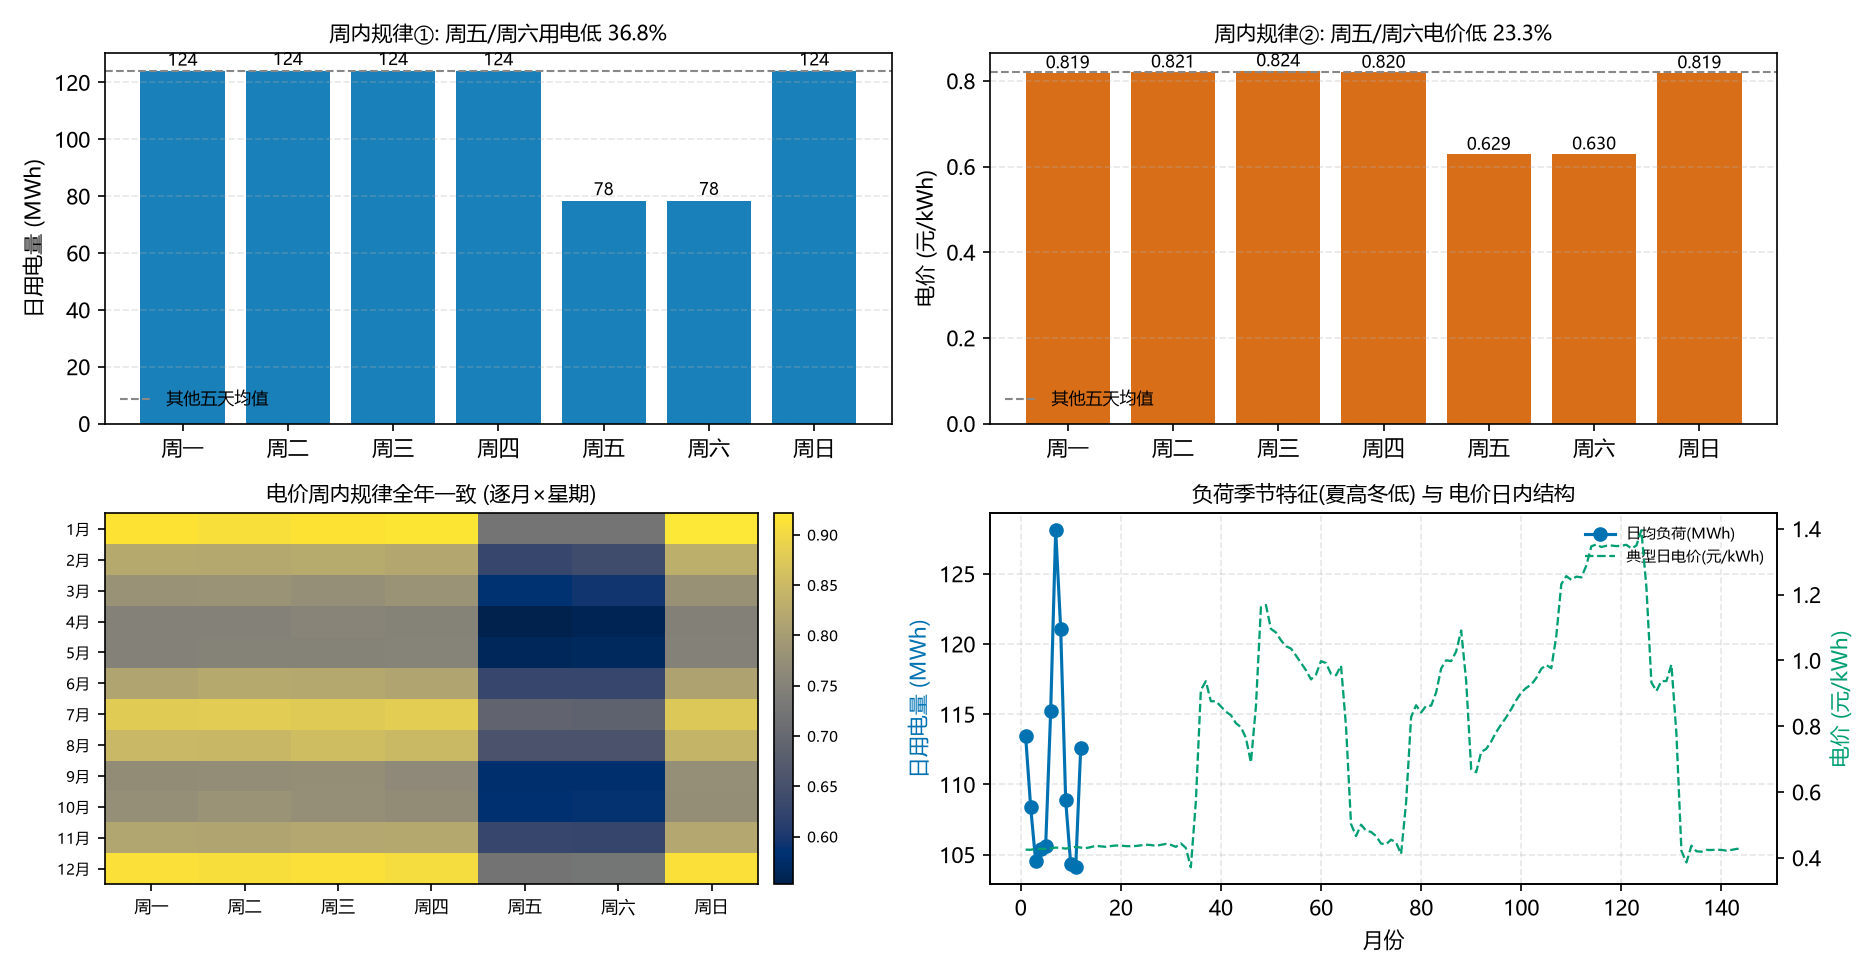
\includegraphics[width=0.92\textwidth]{fig_weekly.png}
\caption{周内规律：日均用电量（左上）、日均电价（右上）、逐月$\times$星期电价热力图（左下）、
负荷季节特征与电价日内结构（右下）}
\label{fig:weekly}
\end{figure}

\begin{figure}[htbp]
\centering
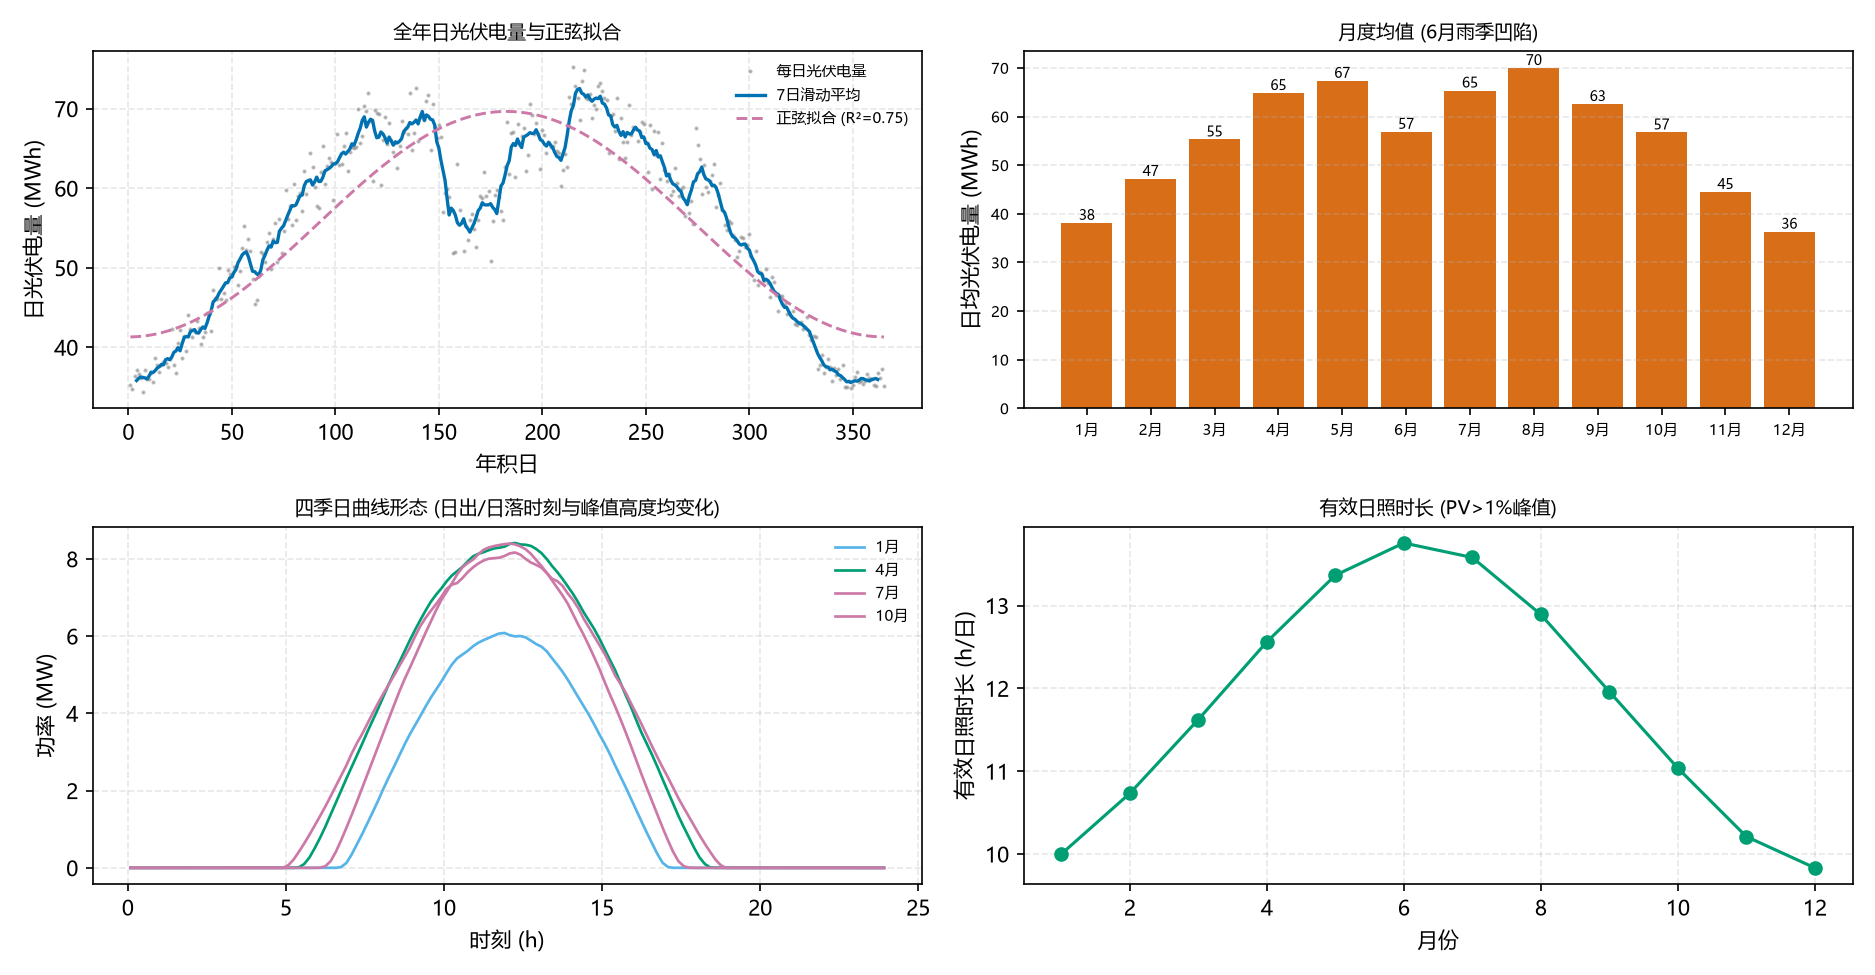
\includegraphics[width=0.92\textwidth]{fig_pv_season.png}
\caption{光伏季节特征：全年日电量与正弦拟合（左上）、月度均值与雨季凹陷（右上）、
四季日曲线形态（左下）、有效日照时长（右下）}
\label{fig:pvseason}
\end{figure}

\subsection{规律四：光伏与负荷噪声的重尾特征}

以“近 4 个同类日平均/近 4 日均值”为基值，净需求残差 $e=e_L-e_P$ 的分布呈现明显
\textbf{重尾}：偏度均值 $+0.16$（近似对称），而\textbf{超额峰度均值 $+5.96$}（正态为 0，
个别时段高达 21）；标准差最大出现在 12 时（112.2 kWh/时段），与正午光伏波动一致。
按月看，光伏基值误差的标准差在春季与雨季最大（MAE 31--35 kWh/时段），12 月最小（12.9）。

\textbf{建模决策（已建模：经验分位缓冲；并证明“形式不重要、水平才重要”）}：安全裕度取
\textbf{近 30 天净残差的 70\% 经验分位}。五组对照实验（\cref{tab:buffer}）显示：
各种更复杂的形式与本文方案的差异都在 $\pm0.6\text{\%}$ 以内
（分噪声叠加 $-0.52\text{\%}$、正态参数化 $+0.58\text{\%}$、60/90 天长窗 $+0.03$/$+0.16\text{\%}$），
而\textbf{分位水平}偏离 0.7 的代价则大得多（$q=0.5$ 时 $+8.27\text{\%}$，见第 \ref{sec:compare} 节）。
其中“分噪声叠加”虽在全年上略优 0.52\%，但它需要\textbf{分别估计负荷与光伏两个误差分布}
（受文献\cite{cqut253,cqut276}“分特征/分时建模、误差不确定性显式计入调度”思想启发），
参数更多，且对\textbf{净需求}的报童问题而言，理论上正确的量正是净残差分位；
本文保留最简且理论更直接的净残差经验分位，把分噪声估计列入第 10 节的改进方向。

\begin{table}[htbp]
\centering
\caption{安全裕度（缓冲）方案的对照实验（全年 2.1--12.31 购电总费用）}
\label{tab:buffer}
\small
\begin{tabular}{@{}lccc@{}}
\toprule
缓冲方案 & 全年总费用(元) & 相对采用 & 结论 \\
\midrule
\textbf{近30天净残差经验分位 $q^*=0.7$（采用）} & \textbf{13\,655\,835} & --- & 最简形式、理论直接 \\
负荷/光伏噪声分别取分位后叠加 & 13\,585\,138 & $-70\,697$ & 参数更多，事后择优 \\
正态参数化（按小时 $\sigma$，$z_{0.7}$） & 13\,734\,664 & $+78\,829$ & 重尾欠覆盖 \\
净残差经验分位（60 天窗） & 13\,659\,929 & $+4\,094$ & 信息陈旧 \\
净残差经验分位（90 天窗） & 13\,677\,410 & $+21\,575$ & 信息陈旧 \\
\bottomrule
\end{tabular}
\end{table}

\subsection{规律五：预测信息价值分解（预言机分析）}

为进一步判断“是否值得为预测噪声投入更复杂的模型”，本文设计\textbf{预言机（oracle）分解}：
分别构造“光伏完全已知”（$PV$ 用实测值，负载仍用预测）与“负载完全已知”（负载用实测值，
光伏仍用预测）两个反事实链条，与采用方案、完全信息下界比较（\cref{fig:noise}）：

\begin{equation}
\underbrace{13\,655\,835}_{\text{采用方案}}
\xrightarrow[\text{光伏噪声价值 }491\,182]{}
\underbrace{13\,164\,653}_{PV\text{完美}}
,\qquad
\underbrace{13\,655\,835}_{\text{采用方案}}
\xrightarrow[\text{负荷噪声价值 }423\,973]{}
\underbrace{13\,231\,862}_{L\text{完美}}
,\qquad
\underbrace{12\,286\,531}_{\text{完全信息下界}} .
\end{equation}

即距完全信息下界的 136.9 万元缺口主要由三部分构成：\textbf{光伏噪声 49.1 万元（35.9\%）、
负荷噪声 42.4 万元（31.0\%）、交互项 33.2\%}。
\textbf{建模决策}：两项噪声的信息价值合计仅 91.5 万元（占总费用 6.7\%），
而且这是“完美预知”的\textbf{理论上限}、不可实现；作为对比，本文的\textbf{实时平衡控制}
在同一条计划下就省下 90.2 万元（相对僵硬执行 $-6.20\text{\%}$），与这一上限同量级。
因此本文\textbf{不引入分布鲁棒优化、机会约束等重装备}，
而是按“先核算信息价值、再决定建模投入”的原则，把建模资源投在\textbf{可实现的实时平衡控制}
与\textbf{低成本高收益的预测模型组合}上（第 \ref{sec:q2} 节）。

\subsection{规律六：预报误差随提前期增长}

附件3 预报的平均绝对误差随提前期增大：0:00 发布为 181.3 kW，6:00 发布 97.4 kW，
12:00 发布 208.1 kW，18:00 发布 260.1 kW（\cref{fig:fcerr}）；同一目标小时在相邻 6 小时
两次预报之间的平均修正幅度为 \textbf{273 kW}。\textbf{建模决策（已建模：滚动调整，且必须“重新定裕度”）}：
Q3 采用滚动时域调整（第~\ref{sec:q3} 节）。实测显示，调整的价值\textbf{完全取决于“该时刻的预报
是否带来新信息”以及“裕度是否随预报重新标定”}——
\textbf{12:00 单次调整值 7.89 万元}（13\,576\,891 元，$-0.58\text{\%}$），
\textbf{6:00 单次调整反而贵 18.39 万元}（$+1.94\text{\%}$，该时刻预报对当日剩余时段几乎无增量），
18:00 调整贵 1.24 万元，全滚动（6/12/18）13\,583\,600 元也不如只调一次。
更关键的是：若在 12:00 调整时\textbf{沿用 0:00 的旧裕度}而不按当日新预报重新标定残差分位，
费用立刻升到 \textbf{14\,704\,403 元（比不调整贵 104.9 万元）}，
说明\textbf{“调整了预报却不调整安全裕度”会让调整彻底失效}（\cref{tab:q3cmp}）。
这与“预报在持续改进”并不矛盾——预报改进的价值首先被更好的 0:00 计划与实时平衡吸收，
调整只在“信息增量大 $+$ 裕度同步更新”时才产生正收益。

\begin{figure}[htbp]
\centering
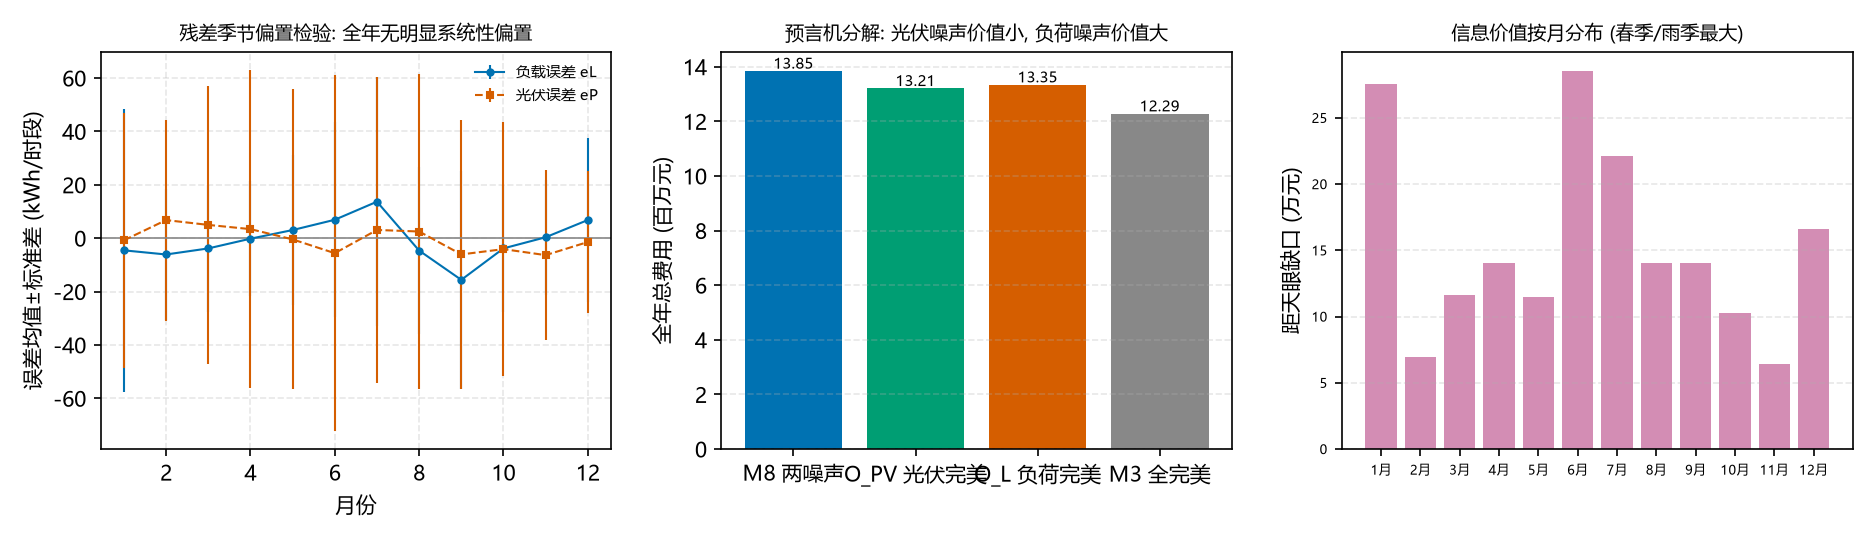
\includegraphics[width=0.95\textwidth]{fig_noise.png}
\caption{噪声与季节性证据：残差逐月均值$\pm$标准差（左）、预言机信息价值分解（中）、
距完全信息下界的缺口按月分布（右）}
\label{fig:noise}
\end{figure}

\begin{figure}[htbp]
\centering
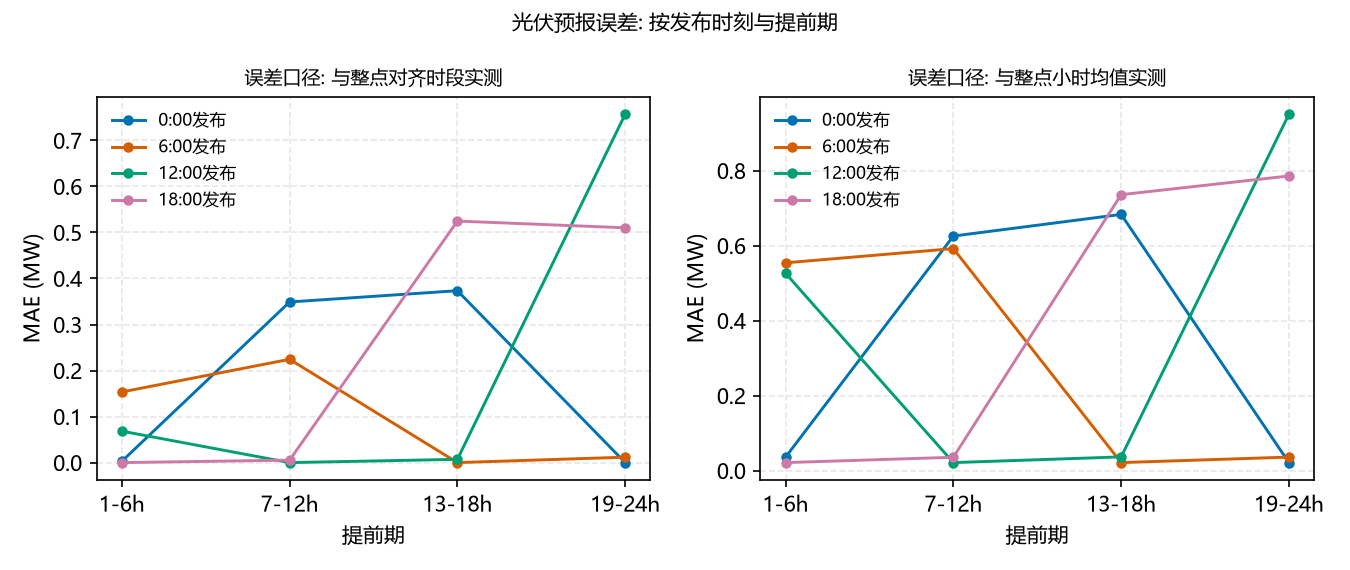
\includegraphics[width=0.85\textwidth]{fig_fcerr.png}
\caption{光伏预报误差：按发布时刻与提前期分桶的平均绝对误差}
\label{fig:fcerr}
\end{figure}

\subsection{规律与建模决策汇总}

\begin{table}[htbp]
\centering
\caption{全部数据规律及其建模决策}
\label{tab:patterns}
\scriptsize
\begin{tabularx}{\textwidth}{@{}p{2.5cm}p{3.6cm}p{2.4cm}X@{}}
\toprule
规律 & 关键数字 & 决策 & 依据/证据 \\
\midrule
周内负荷 & 周五六低 36.8\% & \textbf{已建模并升级}（水平$\times$形状 + 分类凸组合） & 负载 MAE $137.5\to132.3$ kW（周五六 $-8.0\%$），全年 $-36.5\text{\%}$ \\
周内电价 & 周五六低 23.3\% & 不单独建模 & LP 自动利用（周五净充最高）；用预测电价反而 $-0.20\text{\%}$ \\
光伏季节 & 1.93 倍，正弦 $R^2=0.754$，6 月凹陷 & 不单独建模 & 动量修正 $+0.63\text{\%}$；残差无季节偏置；$q^*$ 逐月不变 \\
负荷季节 & 夏高冬低（104--128 MWh/日） & 不单独建模 & 同类日平均残差无季节偏置 \\
噪声重尾 & 峰度 $+5.96$ & \textbf{已建模}（经验分位缓冲） & 复杂缓冲形式差异 $<0.6\text{\%}$；$q=0.5$ 则 $+8.27\text{\%}$ \\
信息价值 & 光伏 35.9\%/负荷 31.0\%/交互 33.2\% & 只做“可实现的改进” & 两项噪声上限 91.5 万，实时平衡已省 90.2 万 \\
预报提前期 & MAE 181$\to$260 kW；更新 273 kW & \textbf{已建模}（滚动调整） & 升级 0:00 依据后调整无正收益（$-28.5\sim+0.3$ 万元） \\
\bottomrule
\end{tabularx}
\end{table}


\section{模型假设与符号说明}
\label{sec:assume}

\subsection{模型假设}

\begin{enumerate}[label=\textbf{假设\arabic*.}, leftmargin=4.2em, itemsep=2pt]
\item 各时段附件给出的功率（kW）为该 10 分钟区间的平均功率，故区间电量（kWh）$=$ 功率 $\times \frac{10}{60}$；
\item 光伏发电优先本地消纳，富余功率可用于储能充电；当富余功率超过储能最大充电功率时允许\textbf{弃光}；
\item 储能充放电效率取\textbf{单程 90\%}（充电存入 90\%、放电放出 90\%，往返 81\%），且同一时段不会同时充放电（LP 最优解自动满足）；
\item 微网与外网的联络线购电能力不受限（无功率上限），但供电不得低于小区负载，缺口须以 5 倍电价紧急购电；
\item 问题二中 0:00 制定计划时\textbf{无法获得当日实测负载与光伏}，只能利用历史实测数据构造预测；
计划量报出后不可更改，日内由储能按第 \ref{sec:q2} 节的\textbf{实时平衡控制规则}兜底
（只用当前实测与当前储电量），兜不住的缺口才按 5 倍电价紧急购电；
\item 问题三中 0:00 计划依据 0:00 发布的光伏预报，6:00/12:00/18:00 的调整仅作用于其后时段并继承当前储电量；
\item 问题四中规划时已知当日实时电价（现货日前市场口径）；
\item 结果文件窗口为 2025-02-01 至 12-31；2025 年 1 月作为储电量链条与预测历史信息的预热期（初始储电量 6000 kWh 对应 2025-01-01 0:00）；
\item 日末储电量以“次日平均电价 $\times$ 放电效率”作为残值计入当日目标函数（滚动时域的标准做法，避免每日耗尽储能的短视行为）；
\item 忽略线路损耗、储能自放电与设备老化，各时段参数在日内不变。
\end{enumerate}

\subsection{符号说明}

\begin{table}[htbp]
\centering
\caption{主要符号}
\label{tab:symbols}
\small
\begin{tabular}{@{}clcl@{}}
\toprule
符号 & 含义 & 符号 & 含义 \\
\midrule
$t$ & 时段序号，$t=1,\dots,144$ & $C_t,D_t$ & 时段 $t$ 的充电量、放电量（kWh）\\
$L_t$ & 时段 $t$ 小区负载电量（kWh） & $E_t$ & 时段 $t$ 起始储电量（kWh）\\
$PV_t$ & 时段 $t$ 光伏发电量（kWh） & $E_0,E_{145}$ & 0:00、24:00 储电量（kWh）\\
$P_t$ & 时段 $t$ 计划购电量（kWh） & $\eta_c,\eta_d$ & 充、放电效率，均取 0.9\\
$p_t$ & 时段 $t$ 电价（元/kWh） & $v$ & 日末储电量残值系数（元/kWh）\\
$q$ & 报童安全裕度的分位水平 & $b_t$ & 时段 $t$ 的安全裕度（kWh）\\
$\hat L_t,\hat{PV}_t$ & 负载、光伏的预测（基值） & $S_t,X_t$ & 计划超出量、调整超出量（kWh）\\
$\bar C,\bar D$ & 充放电功率上限折合 833.33 kWh & $E_t^{\text{急}}$ & 时段 $t$ 紧急购电量（kWh）\\
\bottomrule
\end{tabular}
\end{table}

\subsection{通用单日线性规划模型}

综合第 2 节的机理与第 3 节的规律，四问共用的单日 LP 如下（以预测基值 $\hat L,\hat{PV}$ 为输入）：

\begin{equation}
\underset{P,C,D,E}{\text{min}}\quad \sum_{t=1}^{144} p_t P_t \;-\; v\,E_{145}
\label{eq:obj}
\end{equation}
\begin{align}
\text{s.t.}\quad & \hat{PV}_t + P_t + D_t - C_t \ \ge\ \hat L_t, && t=1,\dots,144 \label{eq:c1}\\
& E_{t+1} = E_t + \eta_c C_t - \frac{D_t}{\eta_d}, && t=1,\dots,144 \label{eq:c2}\\
& 1200 \le E_t \le 10800, && t=1,\dots,145 \label{eq:c3}\\
& 0 \le C_t \le \bar C,\quad 0 \le D_t \le \bar D, && t=1,\dots,144 \label{eq:c4}\\
& P_t \ge 0, && t=1,\dots,144 \label{eq:c5}
\end{align}
其中 $E_1=E_0$ 由链条给出（问题一取 $E_1=E_{145}=6000$；问题二至四取前一日的 24:00 储电量），
残值系数 $v=0.9\times\bar p_{\text{次日}}$（问题一不含残值项而直接约束端点相等）。
该模型为\textbf{标准线性规划}，决策变量 $4\times144+1=577$ 个，约束 $288+1$ 条，
用 HiGHS 内点/单纯形混合算法求解，单日求解时间约 9 ms。


\section{问题一：单典型日确定性最优计划模型}
\label{sec:q1}

\subsection{模型建立}

问题一中电价、负载与光伏预测在 0:00 全部已知，且要求 0:00 与 24:00 储电量相同，
故在通用模型 \eqref{eq:obj}--\eqref{eq:c5} 上取 $\hat L_t=L_t^{\text{附1}}$、
$\hat{PV}_t=PV_t^{\text{附1}}$、$p_t=p_t^{\text{附1}}$，并施加端点约束
\begin{equation}
E_1 = E_{145} = 6000\ \text{kWh},
\label{eq:q1end}
\end{equation}
去掉残值项。该模型共 577 个变量、289 条约束，用 HiGHS 求解约 9 ms，
\textbf{残差最大值 $1.1\times10^{-13}$ kWh}，SOC 全程位于 $[1200,10800]$ 且触及上下限，
无同时充放电时段，说明解在物理上完全可行且约束均被有效利用。

\subsection{求解结果}

\begin{table}[htbp]
\centering
\caption{问题一：指定时段的购电量及全天购电量与购电费（表 1 格式）}
\label{tab:q1a}
\small
\begin{tabular}{@{}lrlrlr@{}}
\toprule
时间段 & 购电量(kWh) & 时间段 & 购电量(kWh) & 时间段 & 购电量(kWh) \\
\midrule
10:00--10:10 & 0.00 & 12:00--12:10 & 480.41 & 14:00--14:10 & 0.00 \\
16:00--16:10 & 445.43 & 18:00--18:10 & 531.89 & 20:00--20:10 & 0.00 \\
\multicolumn{2}{l}{\textbf{全天购电量}} & \multicolumn{4}{l}{\textbf{59\,482.67 kWh}} \\
\multicolumn{2}{l}{\textbf{全天购电费}} & \multicolumn{4}{l}{\textbf{35\,126.95 元}} \\
\bottomrule
\end{tabular}
\end{table}

\begin{table}[htbp]
\centering
\caption{问题一：储能设备分时段充放电量与 0:00、24:00 储电量（表 2 格式）}
\label{tab:q1b}
\small
\begin{tabular}{@{}lrrlrr@{}}
\toprule
时间段 & 充电量(kWh) & 放电量(kWh) & 时间段 & 充电量(kWh) & 放电量(kWh) \\
\midrule
0:00--4:00 & 4500.00 & 0.00 & 4:00--8:00 & 833.33 & 6365.84 \\
8:00--12:00 & 4787.96 & 1703.00 & 12:00--16:00 & 5286.04 & 91.10 \\
16:00--20:00 & 0.00 & 5780.13 & 20:00--24:00 & 5333.33 & 2859.87 \\
\midrule
0:00 储电量 & \multicolumn{2}{r}{6000.00 kWh} & 24:00 储电量 & \multicolumn{2}{r}{6000.00 kWh} \\
\bottomrule
\end{tabular}
\end{table}

\begin{figure}[htbp]
\centering
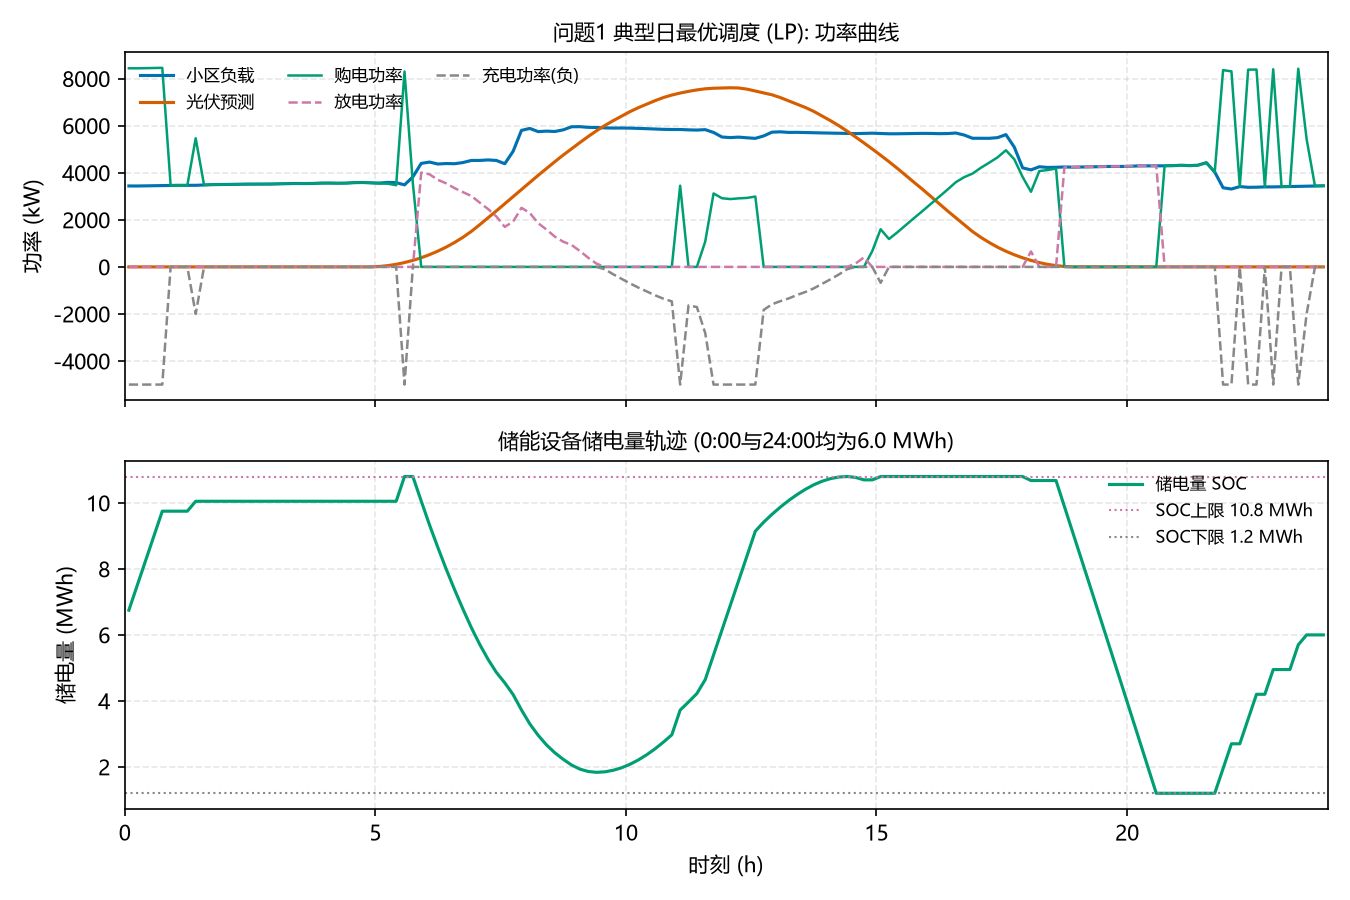
\includegraphics[width=0.86\textwidth]{fig_q1_schedule.png}
\caption{问题一最优调度：功率曲线（上）与储电量轨迹（下）}
\label{fig:q1}
\end{figure}

\subsection{结果分析}

最优策略呈现清晰的“低充高放”结构（\cref{fig:q1}、\cref{tab:q1a}、\cref{tab:q1b}）：

\begin{enumerate}[label=(\arabic*), leftmargin=2.2em, itemsep=1pt]
\item \textbf{夜间低价充电（0:00--4:00，电价均值 0.432 元/kWh）}：充电 4500 kWh 将储电量由 6000 抬升至 10\,050 kWh；
\item \textbf{早高峰放电（4:00--8:00，电价均值 0.671 元/kWh）}：放电 6365.84 kWh 覆盖负载高峰，
其边际成本 $0.432/0.81=0.533$ 元/kWh 低于直接购电；
\item \textbf{午间弃光充电（8:00--16:00）}：光伏富余功率为免费电源，共充电 10\,074 kWh；
\item \textbf{傍晚尖峰放电（16:00--20:00，电价均值 1.134 元/kWh）}：放电 5780.13 kWh 是全天收益最高的动作；
\item \textbf{夜间回充并精准归位}：20:00--24:00 充电 5333.33 kWh，使 24:00 储电量恰好回到 6000 kWh，
满足端点约束的同时用尽低价时段。
\end{enumerate}

\subsection{方法对照：LP 与启发式、与无储能基线}

\begin{table}[htbp]
\centering
\caption{问题一三种方法的对照（典型日购电费）}
\label{tab:q1cmp}
\small
\begin{tabular}{@{}lccc@{}}
\toprule
方法 & 购电费(元) & 相对 LP & 说明 \\
\midrule
\textbf{线性规划（采用）} & \textbf{35\,126.95} & --- & 577 变量精确最优，9 ms \\
贪心配对启发式 & 42\,187.93 & +7\,060.98 (+20.1\%) & 忽略充放电时序约束的松弛解 \\
无储能基线 & 48\,052.05 & +12\,925.10 (+36.8\%) & 缺额全部按当时电价购买 \\
\bottomrule
\end{tabular}
\end{table}

\cref{tab:q1cmp} 表明：储能使典型日购电费下降 \textbf{26.9\%}（12\,925 元）；
而启发式即便在“忽略时序约束”的宽松条件下仍比 LP 贵 7061 元，
印证了第 2 节“本问题应当用 LP 精确求解”的判断。


\section{问题二：全年逐日“计划—结算”两阶段模型}
\label{sec:q2}

\subsection{信息结构与我方预测模型}

问题二要求“在每天 0:00 制定当天的计划购电策略”，而 0:00 显然无法获得当日实测数据，
因此计划必须建立在\textbf{由历史实测（与 0:00 已发布的附件3 预报）构造的预测}之上，
当日实测数据只用于\textbf{结算}。结合第 3 节的周内规律（周五、周六用电低 36.8\%），
本文构造了一组\textbf{可分解、可堆叠}的预测模型，并用同一套因果管道逐项验证
（全部超参只在 1 月标定，2--12 月为外样本）。

\textbf{（1）负载预测：水平$\times$形状分解 + 分类组合}。记第 $d$ 天第 $t$ 时段负载为 $L_d(t)$。
把“日总量（水平）”与“日内曲线（形状）”分开建模：
\begin{equation}
L_d(t)=\underbrace{\Lambda_d}_{\text{水平}}\cdot\underbrace{\sigma_{c(d)}(t)}_{\text{形状}},\qquad
\Lambda_d=\frac{1}{4}\sum_{\tau\in H_d}\sum_{t}L_\tau(t),
\label{eq:basisL}
\end{equation}
其中 $H_d$ 为最近 4 个\textbf{同类日}（周五、周六记为“低”类 $c(d)=\text{L}$，其余五天记为“高”类），
$\sigma_{c}(t)$ 为同类日近 6 天归一化曲线（$L/\sum_tL$）的均值。
另构造\textbf{递推水平平滑}（对“昨日实际/预测总量比”做指数平滑，$\alpha=0.35$，限幅 $[0.85,1.15]$）
与\textbf{全局误差反馈}（近 3 日实测/预测比阻尼校正）两个候选，最后\textbf{按两类分别做凸组合}，
权重在 1 月标定集上网格搜索：
\begin{equation}
\hat L_d(t)=\sum_{k=1}^{4}w^{c(d)}_k\,g_k(t),\qquad
w^{\text{L}}=(0,\,0.3,\,0.7,\,0),\quad w^{\text{H}}=(0,\,1.0,\,0,\,0),
\label{eq:loadweights}
\end{equation}
即\textbf{周五/周六以“递推水平$\times$同类形状”为主（0.7），其余五天用“同类日水平$\times$形状”（1.0）}。
该结构使两类日子的误差同时下降（见 \cref{tab:fcacc}），这是“不分周五六的稳健统计”
（近 5 日中位数、近 5 日加权平均）误差高达 652$\sim$1056\,kW 的反证。

\textbf{（2）光伏预测：因果岭回归堆叠}。以 4 个基模型为输入：
近 4 日均值 $b_1$、误差反馈 $b_2$（近 2 日实测/预测比阻尼校正）、
LightGBM $b_3$（30 维特征：时段、星期、年内谐波、滞后与滚动的光伏/负载/电价、附件3 预报）、
以及\textbf{附件3 的 0:00 发布预报} $b_4$；用带时段与类别交互项的\textbf{岭回归}在历史样本上
（每 14 天用截至当时的样本重训，保证因果）学习最优权重：
\begin{equation}
\widehat{PV}_d(t)=\beta_0+\sum_{k=1}^{4}\beta_k\,b_k(t)+\beta_5\tau+\beta_6\mathbb{1}_{\text{L}}
+\beta_7\tau\mathbb{1}_{\text{L}},\qquad
\bm\beta=\arg\min_{\bm\beta}\sum_{j<d}\sum_t\Big(\sum_k\beta_kb_k^{(j)}(t)+\cdots-PV_j(t)\Big)^2+\alpha\|\bm\beta\|^2 .
\label{eq:basisPV}
\end{equation}
单模型都不如“近 4 日均值”（附件3 预报 206.7\,kW、晴空指数模型 213.3\,kW、
LightGBM 151.2\,kW、近 4 日均值 152.0\,kW），
但\textbf{堆叠后 MAE 降到 136.9\,kW（$-9.9\%$）}——收益来自多源信息的最优组合。

\textbf{（3）实时电价预测（用于第 \ref{sec:q4} 节的“未知电价”情形）}：
先取同类日近 6 天同槽位中位数作廓线、并按最近同类日水平做自适应缩放，
再与廓线误差反馈、LightGBM 做同样的因果岭回归堆叠，MAE 由同类日均价的 0.0581
降到 \textbf{0.0367 元/kWh}。

\begin{table}[htbp]
\centering
\caption{预测模型精度对照（2.1--12.31 外样本，单位：负荷/光伏 kW、电价 元/kWh）}
\label{tab:fcacc}
\scriptsize
\begin{tabular}{@{}llccc@{}}
\toprule
对象 & 模型 & MAE & RMSE & 日总量 MAPE \\
\midrule
\multirow{5}{*}{负载}
& 近 4 个同类日均值（原依据） & 137.52 & 191.59 & 1.06\% \\
& 指数加权同类日（8 日，0.85） & 140.45 & 196.61 & 1.36\% \\
& 相似日 kNN（5 个同类日） & 286.99 & 448.43 & 4.76\% \\
& 岭回归 / LightGBM（逐时段特征） & 188.58 / 159.32 & 283.72 / 259.71 & 2.77\% / 1.73\% \\
& \textbf{水平$\times$形状 + 分类凸组合（采用）} & \textbf{132.28} & \textbf{182.24} & \textbf{0.94\%} \\
\midrule
\multirow{5}{*}{光伏}
& 近 4 日均值（原依据） & 151.95 & 307.33 & 3.64\% \\
& 附件3 的 0:00 预报 & 206.65 & 388.78 & 5.27\% \\
& 晴空指数模型（近 10 日 $k\times$包络） & 213.33 & 384.00 & 3.53\% \\
& LightGBM（30 维特征） & 151.24 & 302.57 & 4.14\% \\
& \textbf{因果岭回归堆叠（采用）} & \textbf{136.85} & \textbf{261.74} & \textbf{3.49\%} \\
\midrule
\multirow{3}{*}{电价}
& 同类日近 30 日均价 & 0.0581 & --- & 1.75\% \\
& 廓线 + 自适应水平 / LightGBM & 0.0372 / 0.0370 & 0.052 / 0.053 & 1.75\% / 1.85\% \\
& \textbf{因果岭回归堆叠（采用）} & \textbf{0.0367} & \textbf{0.050} & 1.86\% \\
\midrule
\multicolumn{2}{@{}l}{负载分类精度（采用 vs 原依据）} & 周五六 142.21 / 154.60 & 其他五天 128.33 / 130.73 & 见正文 \\
\bottomrule
\end{tabular}
\end{table}

\textbf{（4）报童安全裕度}。定义净需求预测残差
$e_d(t)=\big(L_d(t)-\hat L_d(t)\big)-\big(PV_d(t)-\widehat{PV}_d(t)\big)$，
计划所用的“计划净需求”为预测加裕度：
\begin{equation}
\tilde N_d(t)=\hat L_d(t)-\widehat{PV}_d(t)+b_d(t),\qquad
b_d(t)=\mathrm{Quantile}_{q}\big(\{e_\tau(t)\}_{\tau\in\text{近30天}}\big).
\label{eq:buffer}
\end{equation}
分位水平 $q$ 由报童模型\cite{newsboy}确定：购电偏少的额外代价为紧急电价与基准电价之差 $c_u=5p-p=4p$，
购电偏多的代价为基准电价 $c_o=p$，故理论最优服务水平
\begin{equation}
q^*=\frac{c_u}{c_u+c_o}=\frac{4p}{4p+p}=0.8 .
\label{eq:newsboy}
\end{equation}
但由于日内实时平衡控制已能吸收大部分意外偏差，实测最优分位低于理论值：在 1 月标定集上
\begin{equation}
\mathrm{Cost}_{1\text{月}}(q=0.5/0.6/\textbf{0.7}/0.8/0.9)
=1\,282\,669\,/\,1\,244\,876\,/\,\bm{1\,237\,127}\,/\,1\,252\,414\,/\,1\,317\,816\ \text{元},
\label{eq:qtune}
\end{equation}
故取 $\bm{q^*=0.7}$，并在 2--12 月做外样本评估；储能放电下限取物理下限
$\underline E=1200$ kWh（第 \ref{sec:compare} 节给出裕度形式与分位水平的敏感性）。

\subsection{计划模型与结算模型（分开建模）}

\textbf{（1）0:00 计划模型}。以 $\tilde N_d$ 为输入求解式 \eqref{eq:obj}--\eqref{eq:c5}
（其中 $\hat L$ 替换为 $\hat L+b$、$\widehat{PV}$ 替换为预测值），得到计划购电量 $P^0_t$
与计划充放电量 $C^0_t,D^0_t$，并给出计划储电量轨迹 $E^0_t$。

\textbf{（2）日内结算模型：实时平衡控制}。计划报出后\textbf{购电量 $P^0_t$ 不再改变}
（否则等于允许“事后修改计划”），但储能是微网内部可控设备，题面又要求
“微网提供的电能不可低于小区负载”，因此运行中必须用储能\textbf{实时兜底}。
本文把这一过程写成\textbf{逐时段因果控制规则}：时段 $t$ 的决策只使用当前时刻可获得的量
（当前实测 $L_t,PV_t$、当前储电量 $E_t$ 与已锁定计划），\textbf{不使用任何未来实测}。

需要特别强调：\textbf{问题二只有 0:00 一个决策时刻}。上面这条规则并非“日内重新优化”，
而是与计划 $(P^0,C^0,D^0)$ \textbf{同时}在 0:00 就确定下来、并写入策略的一条\textbf{响应规则}
（式 \eqref{eq:clip}--\eqref{eq:socrec} 中不含任何未来信息，也不需要在线求解任何优化问题，
只是把偏差按“先动用计划充放电的可调空间、再动用储能存量、最后才紧急购电”的优先级消化）。
换言之，本文的 0:00 决策输出的是\textbf{“购电计划 $+$ 储能响应规则”这一对}
（相当于一个状态反馈策略 $\pi_t(\cdot)$），日内不产生任何新的、免费的调整机会；
若不采用该规则而僵硬照表执行（缺口一律按 $5p_t$ 紧急购电），全年费用将升至 14\,557\,730 元
（\cref{tab:q2exec}），这正是该规则的价值所在。

记 $\bar C=833.33$ kWh/10\,min（5000 kW）、$\eta_c=\eta_d=0.9$、
储电量上下限 $\underline{E}=1200,\ \overline{E}=10800$ kWh。控制规则为：

\textbf{① 可行性裁剪}：把计划充放电量裁剪到当前状态可达范围
\begin{equation}
C^{o}_t=\text{min}\Big\{\text{max}(C^0_t,0),\ \bar C,\ \frac{\overline{E}-E_t}{\eta_c}\Big\},\qquad
D^{o}_t=\text{min}\Big\{\text{max}(D^0_t,0),\ \bar C,\ \eta_d\big(E_t-\underline{E}+\eta_cC^{o}_t\big)\Big\}.
\label{eq:clip}
\end{equation}

\textbf{② 计划口径缺口}：$\Delta_t=L_t-\big(PV_t+P^0_t+D^{o}_t-C^{o}_t\big)$。
若 $\Delta_t>0$（实际比计划“更缺电”），先\textbf{少充}、再\textbf{多放}：
\begin{align}
C_t&=\text{max}\big(0,\ C^{o}_t-\Delta_t\big),\qquad
\Delta'_t=\text{max}\big(0,\ \Delta_t-C^{o}_t\big),\label{eq:up1}\\
D_t&=D^{o}_t+\text{min}\Big\{\Delta'_t,\ \bar C-D^{o}_t,\ \eta_d\big(E_t-\underline{E}+\eta_cC_t\big)-D^{o}_t\Big\},\qquad
E^{\text{急}}_t=\text{max}\big(0,\ \Delta'_t-(D_t-D^{o}_t)\big).\label{eq:up2}
\end{align}
即\textbf{先动用计划充放电的可调空间，再动用储能存量}；仍兜不住的缺口
$E^{\text{急}}_t$ 只能按 $5p_t$ 紧急购电。

\textbf{③ 计划口径富余}：若 $\Delta_t<0$，先\textbf{少放}、再\textbf{多充}：
\begin{align}
D_t&=\text{max}\big(0,\ D^{o}_t+\Delta_t\big),\qquad
\Delta''_t=\text{min}\big(0,\ \Delta_t+D^{o}_t\big),\label{eq:dn1}\\
C_t&=C^{o}_t+\text{min}\Big\{-\Delta''_t,\ \bar C-C^{o}_t,\
\frac{\overline{E}-E_t+D_t/\eta_d}{\eta_c}-C^{o}_t\Big\},\label{eq:dn2}
\end{align}
剩余富余 $\big(-\Delta''_t-(C_t-C^{o}_t)\big)$ 由\textbf{弃光}吸收（题面允许光伏未上网部分直接丢弃）。

最后按
\begin{equation}
E_{t+1}=E_t+\eta_cC_t-\frac{D_t}{\eta_d}
\label{eq:socrec}
\end{equation}
递推储电量。可证式 \eqref{eq:clip}--\eqref{eq:socrec} 自动满足
$C_t,D_t\in[0,\bar C]$、$E_t\in[\underline E,\overline E]$ 与“不同时充放电”三项物理约束
（数值实现中亦以断言逐时段校验），且\textbf{所有量均为 $t$ 时刻已知}，故该规则是
\textbf{可实行的（online、因果）}。当日费用为
\begin{equation}
\text{Cost}_d=\sum_t p_tP^0_t+\sum_t 5p_tE^{\text{急}}_t ,
\label{eq:q2cost}
\end{equation}
储电量链条 $E_{145}^{(d)}=E_1^{(d+1)}$ 逐日递推，1 月为预热期，结果自 2 月 1 日起输出。

\textbf{（3）为什么“分开建模”是必要的}。若把两个阶段合并为一个“事后最优”模型
（用当日实测重新优化储能），等于允许 0:00 决策使用未来信息，得到的是\textbf{不可实行的}
下界而非策略。本文的“计划（历史信息）$+$ 实时平衡（当前信息）”结构下，
决策者的信息集随时间单调增长，不存在事后调整空间。
作为对照（\cref{tab:q2exec}）：若\textbf{僵硬执行}计划，全年费用升至 14\,557\,730 元；
实时平衡控制把它降到 \textbf{13\,655\,835 元（$-6.2\text{\%}$）}；
而“完美信息再调度”（不可实行）为 13\,368\,722 元。

\begin{table}[htbp]
\centering
\caption{问题二：同一计划下三种执行／结算方式的全年费用对照（2.1--12.31）}
\label{tab:q2exec}
\small
\begin{tabular}{@{}llccc@{}}
\toprule
执行方式 & 是否可实行 & 计划购电费(元) & 紧急购电费(元) & 总费用(元) \\
\midrule
僵硬执行计划（无日内平衡） & 可实行 & 12\,862\,043 & 1\,695\,687 & 14\,557\,730 \\
\textbf{实时平衡控制（采用）} & \textbf{可实行} & \textbf{12\,866\,999} & \textbf{788\,836} & \textbf{13\,655\,835} \\
完美信息再调度（事后最优） & 否（需未来实测） & 12\,866\,999 & 501\,723 & 13\,368\,722 \\
\bottomrule
\end{tabular}
\end{table}

\begin{figure}[htbp]
\centering
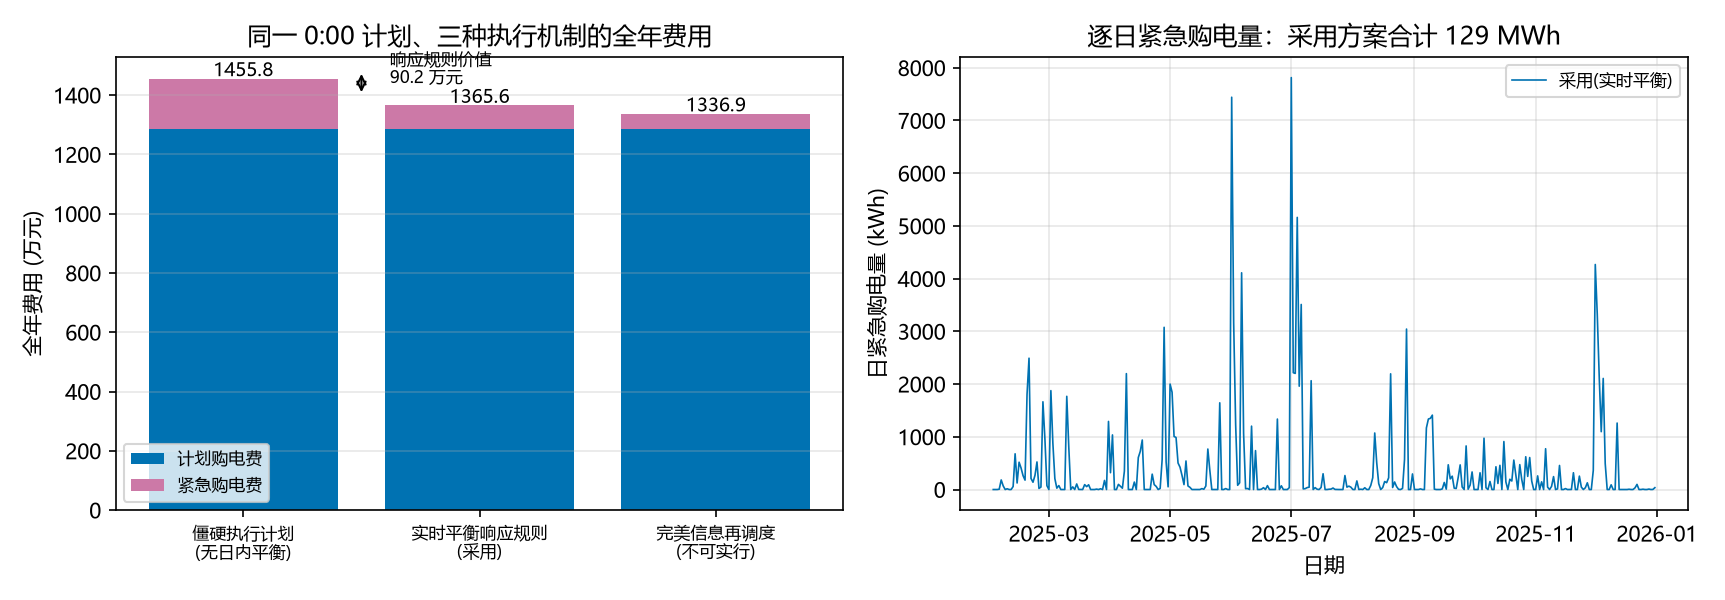
\includegraphics[width=0.95\textwidth]{fig_q2_exec.png}
\caption{同一 0:00 计划下三种执行机制的全年费用分解（左）与采用方案的逐日紧急购电量（右）：
“0:00 定下的响应规则”把紧急购电费由 169.6 万元压到 78.9 万元}
\label{fig:q2exec}
\end{figure}

\subsection{全年结果}

\begin{table}[htbp]
\centering
\caption{问题二全年（2025-02-01 至 12-31，334 天）各方法对照
（全部方法采用同一实时平衡控制结算）}
\label{tab:q2cmp}
\scriptsize
\begin{tabular}{@{}lcccccl@{}}
\toprule
方法（0:00 计划依据） & 计划购电费(元) & 紧急购电费(元) & 总费用(元) & 紧急电量(kWh) & 相对采用 & 说明 \\
\midrule
\textbf{升级预测模型（采用）} & \textbf{12\,866\,999} & \textbf{788\,836} & \textbf{13\,655\,835} & \textbf{129\,289} & --- & 本文方法 \\
原依据（近 4 个同类日均值 $+$ 近 4 日光伏） & 12\,932\,582 & 915\,601 & 13\,848\,183 & 150\,493 & $+1.41\text{\%}$ & 仅换预测依据 \\
附件1 典型日曲线 + 报童 $q=0.7$ & 14\,971\,784 & 3\,346\,902 & 18\,318\,686 & 546\,489 & $+34.1\text{\%}$ & 忽略日际变化 \\
无储能（升级预测+报童） & 18\,155\,061 & （含于左） & 18\,155\,061 & --- & $+32.9\text{\%}$ & 储能价值对照 \\
昨日外推 + 报童 $q=0.6$ & 12\,872\,034 & 8\,619\,722 & 21\,491\,755 & 1\,615\,300 & $+57.4\text{\%}$ & 仅用昨日信息 \\
昨日外推 + 报童 $q=0.8$ & 14\,456\,337 & 7\,333\,092 & 21\,789\,429 & 1\,350\,662 & $+59.6\text{\%}$ & 裕度过大 \\
昨日外推（无裕度） & 12\,296\,521 & 10\,219\,271 & 22\,515\,792 & 1\,887\,772 & $+64.9\text{\%}$ & 朴素外推 \\
两阶段随机规划 SAA（近 20 日情景） & 8\,752\,681 & 31\,201\,329 & 39\,954\,010 & 6\,928\,843 & $+192.6\text{\%}$ & 见第~\ref{sec:compare} 节失效分析 \\
完全信息下界（天眼链式） & 12\,286\,531 & 0 & 12\,286\,531 & 0 & $-10.0\text{\%}$ & 不可达下界 \\
\bottomrule
\end{tabular}
\end{table}

由\cref{tab:q2cmp} 可得三点结论：

\begin{enumerate}[label=(\arabic*), leftmargin=2.4em, itemsep=1pt]
\item \textbf{预测模型的精度是本题最大的杠杆}：把“昨日外推”升级为“水平$\times$形状分解 +
分类组合 + 光伏堆叠”，全年费用由 21\,491\,755 元降至 \textbf{13\,655\,835 元（下降 36.5\%）}，
紧急购电量由 1.62 GWh 降至 0.13 GWh；负载预测 MAE 由 650.0 kW 降到 132.3 kW（$-79.6\text{\%}$），
光伏 MAE 由 307.3（RMSE）对应的 152.0 kW 降到 136.9 kW。
\item \textbf{报童裕度必须与预测依据联合标定}：裕度形式（净残差经验分位 / 正态参数化 /
分噪声叠加 / 60--90 天长窗）差异在 $-0.5\%\sim+0.6\%$ 之间，
而\textbf{分位水平}偏离 0.7 的代价大得多（$q=0.5$ 时 $+8.3\text{\%}$，\cref{tab:sens}）。
\item \textbf{储能价值显著}：无储能时全年 18\,155\,061 元，储能可节约
\textbf{449.9 万元（24.8\%）}；距完全信息下界 136.9 万元，
说明本文方法已接近该信息结构下的效率前沿。
\end{enumerate}

\begin{figure}[htbp]
\centering
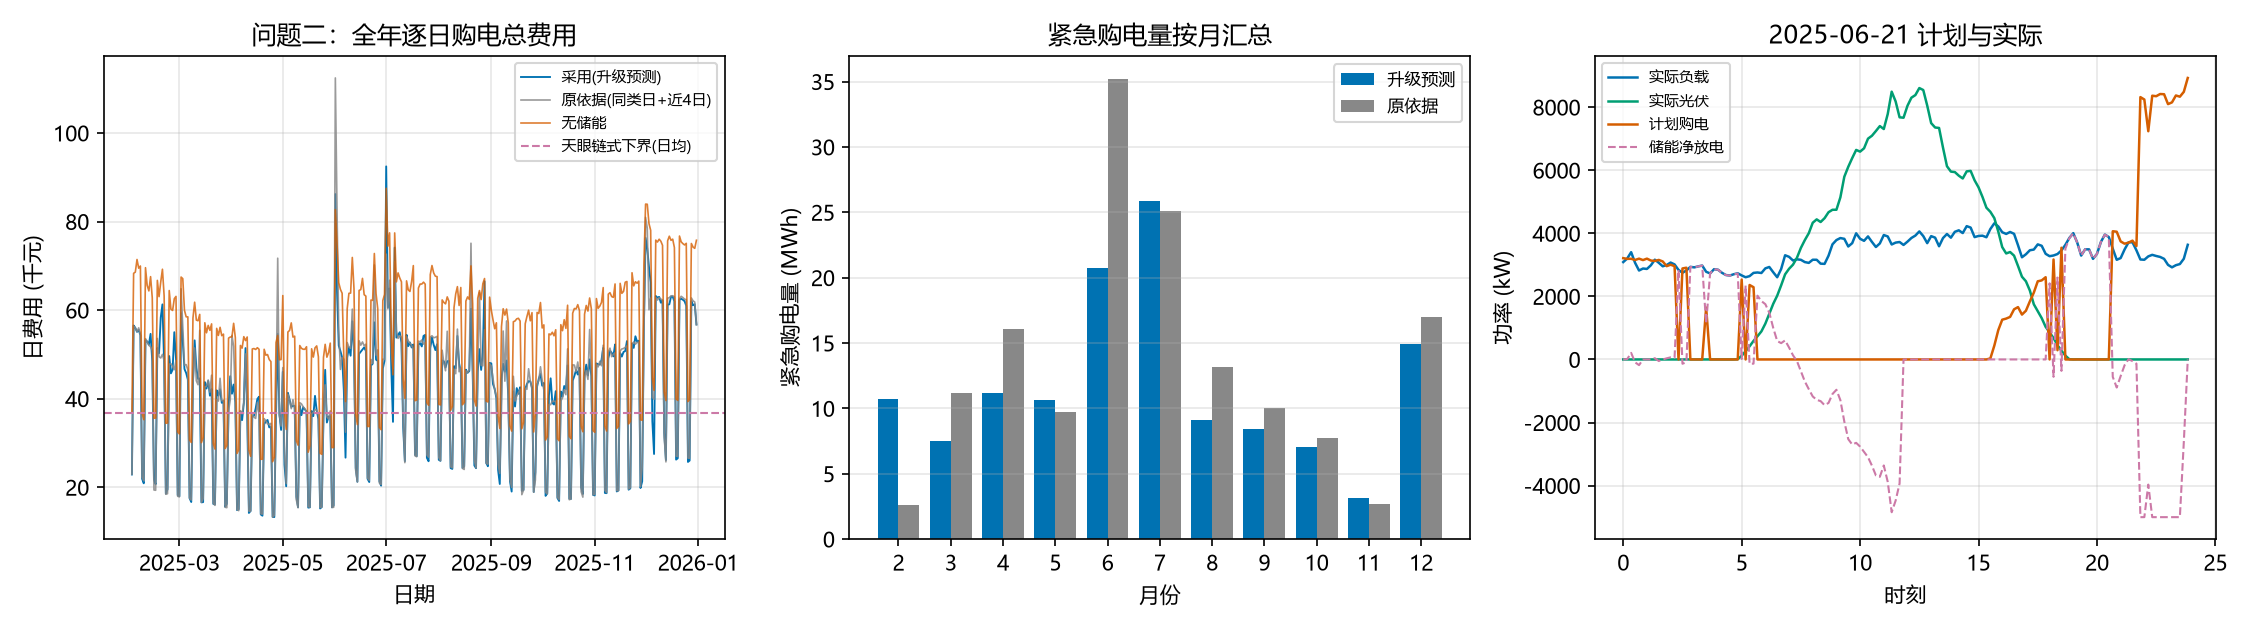
\includegraphics[width=0.95\textwidth]{fig_q2_annual.png}
\caption{问题二：全年逐日购电总费用对比（左）、紧急购电量按月汇总（中）、
2025-06-21 计划与实际（右）}
\label{fig:q2}
\end{figure}

\begin{figure}[htbp]
\centering
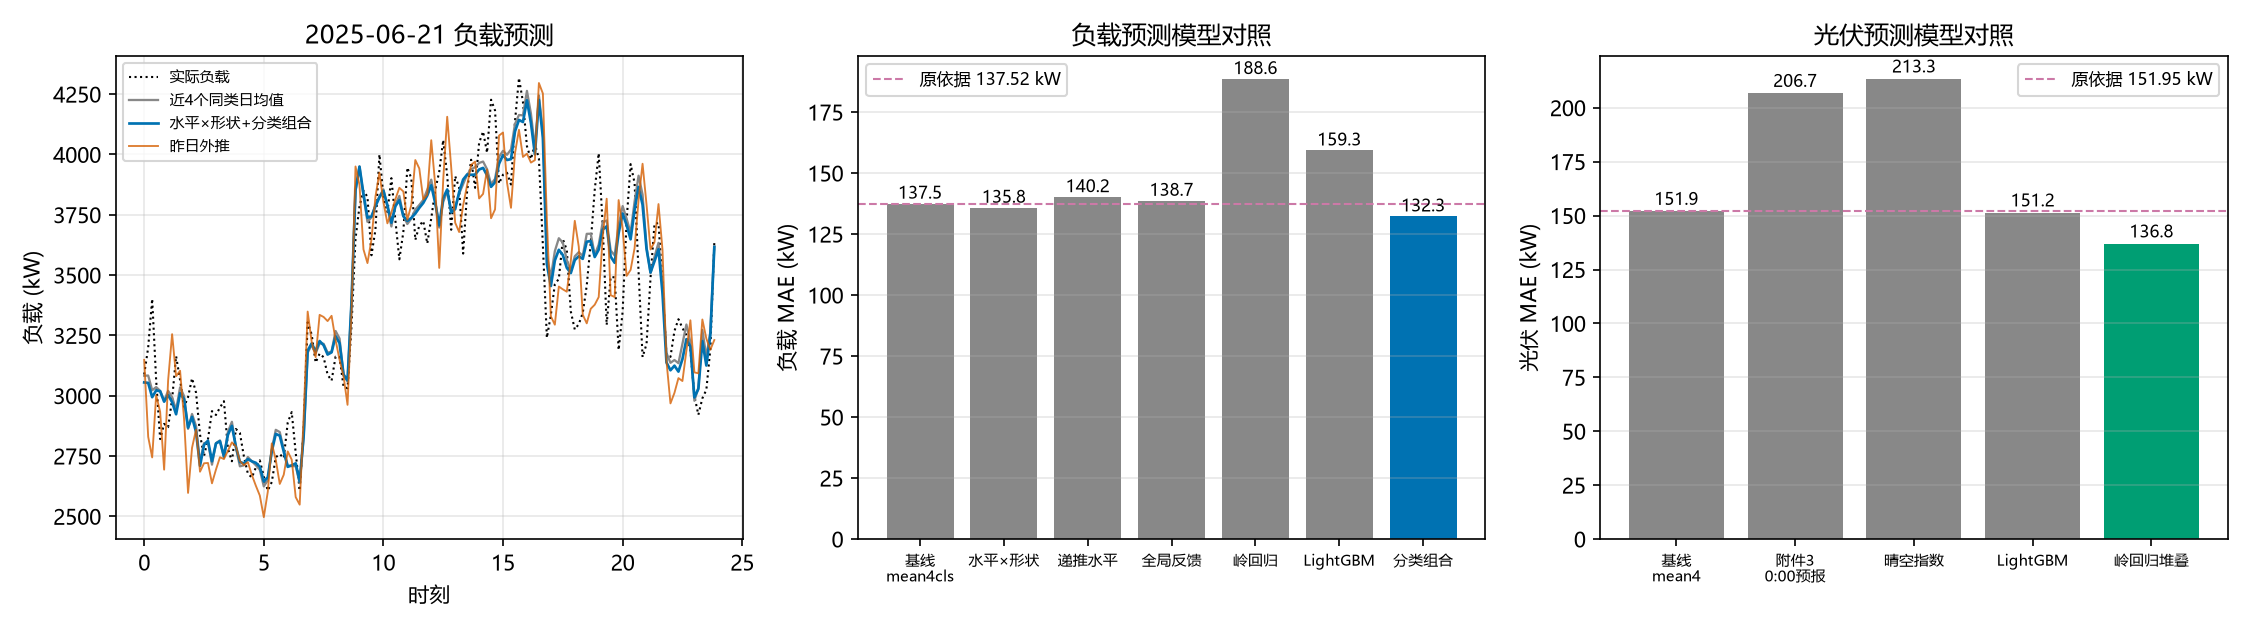
\includegraphics[width=0.62\textwidth]{fig_q2_basis.png}
\caption{预测模型对照：分类组合负荷模型与岭回归堆叠光伏模型的精度优势}
\label{fig:q2basis}
\end{figure}

\begin{figure}[htbp]
\centering
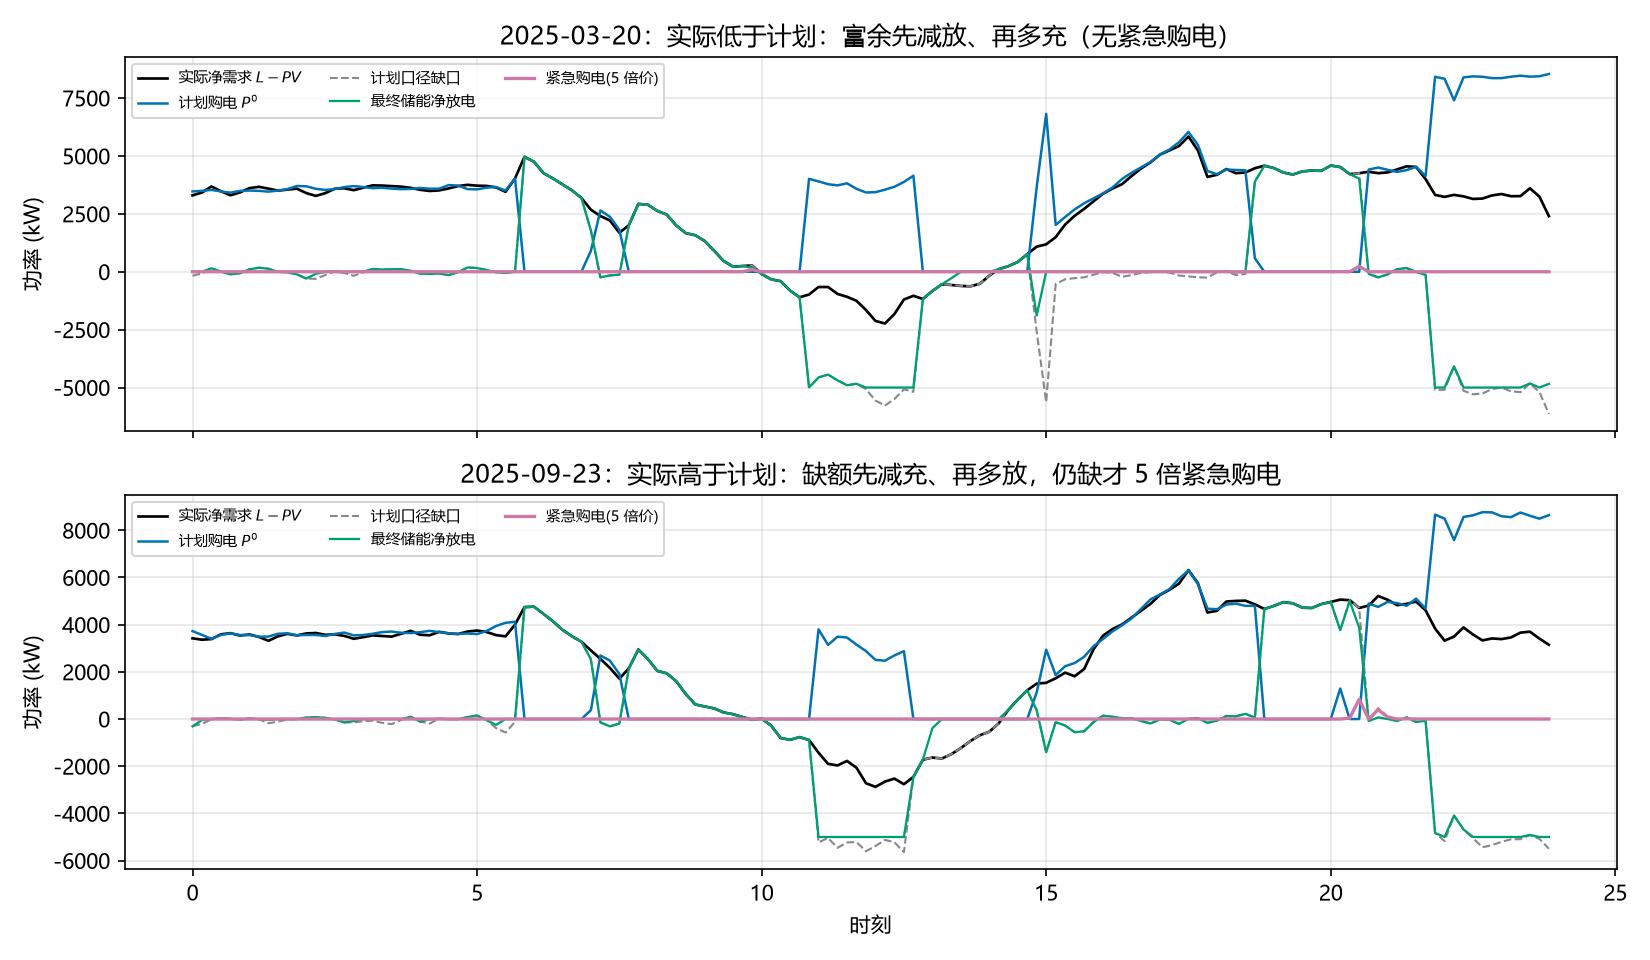
\includegraphics[width=0.95\textwidth]{fig_q2_balance.png}
\caption{实时平衡控制过程：上行（03-20）计划偏保守、储能吸收富余；下行（09-23）实际高于计划、
储能兜底后仍有少量紧急购电}
\label{fig:q2balance}
\end{figure}

\subsection{指定日期结果（表 1、表 2、表 3 格式）}

\begin{table}[htbp]
\centering
\caption{问题二：指定日期关键时段计划购电量与全天购电量、购电费（表 1 格式，kWh/元）}
\label{tab:q2t1}
\scriptsize
\begin{tabular}{@{}lcccc@{}}
\toprule
时间段 & 2025-03-20 & 2025-06-21 & 2025-09-23 & 2025-12-21 \\
\midrule
10:00--10:10 & 0.00 & 0.00 & 0.00 & 0.00 \\
12:00--12:10 & 572.73 & 0.00 & 417.97 & 970.56 \\
14:00--14:10 & 0.00 & 0.00 & 0.00 & 0.00 \\
16:00--16:10 & 564.40 & 210.12 & 565.82 & 847.33 \\
18:00--18:10 & 702.62 & 0.00 & 775.60 & 716.85 \\
20:00--20:10 & 0.00 & 0.00 & 0.00 & 0.00 \\
\midrule
全天购电量 & 69\,247.84 & 37\,122.93 & 68\,471.78 & 97\,053.33 \\
全天购电费 & 41\,846.37 & 21\,173.98 & 42\,566.71 & 62\,140.33 \\
\bottomrule
\end{tabular}
\end{table}

\begin{table}[htbp]
\centering
\caption{问题二：指定日期最终储能充放电量与 0:00、24:00 储电量（表 2 格式，kWh）}
\label{tab:q2t2}
\scriptsize
\begin{tabular}{@{}lcccccccc@{}}
\toprule
\multirow{2}{*}{时间段} & \multicolumn{2}{c}{2025-03-20} & \multicolumn{2}{c}{2025-06-21} &
\multicolumn{2}{c}{2025-09-23} & \multicolumn{2}{c}{2025-12-21} \\
\cmidrule(lr){2-3}\cmidrule(lr){4-5}\cmidrule(lr){6-7}\cmidrule(lr){8-9}
& 充电 & 放电 & 充电 & 放电 & 充电 & 放电 & 充电 & 放电 \\
\midrule
0:00--4:00 & 120.41 & 177.57 & 90.73 & 3628.48 & 110.84 & 58.65 & 72.60 & 100.04 \\
4:00--8:00 & 169.32 & 5935.75 & 389.36 & 4839.09 & 178.05 & 6091.11 & 854.59 & 1456.11 \\
8:00--12:00 & 6028.92 & 2761.36 & 9973.71 & 0.00 & 5607.93 & 1896.62 & 5592.70 & 7159.56 \\
12:00--16:00 & 4952.21 & 254.72 & 0.00 & 0.00 & 4598.44 & 465.74 & 7080.82 & 2300.86 \\
16:00--20:00 & 4.10 & 5751.77 & 151.96 & 5590.59 & 125.58 & 5749.56 & 4.34 & 5832.12 \\
20:00--24:00 & 10\,722.55 & 2936.83 & 9820.78 & 2487.33 & 10\,646.53 & 2956.95 & 10\,666.67 & 2811.39 \\
\midrule
0:00 储电量 & \multicolumn{2}{c}{10\,800.00} & \multicolumn{2}{c}{10\,800.00} &
\multicolumn{2}{c}{10\,747.68} & \multicolumn{2}{c}{10\,800.00} \\
24:00 储电量 & \multicolumn{2}{c}{10\,800.00} & \multicolumn{2}{c}{10\,800.00} &
\multicolumn{2}{c}{10\,756.51} & \multicolumn{2}{c}{10\,800.00} \\
\bottomrule
\end{tabular}
\end{table}

\begin{table}[htbp]
\centering
\caption{问题二：指定日期紧急购电时间段与购电量（表 3 格式，kWh）}
\label{tab:q2t3}
\scriptsize
\begin{tabular}{@{}llll@{}}
\toprule
2025-03-20（合计 54.68） & 2025-06-21 & 2025-09-23（合计 228.74） & 2025-12-21（合计 31.13） \\
\midrule
9:50--10:00\ 16.02 & \multicolumn{1}{c}{无紧急购电} & 20:20--20:40\ 145.79 & 20:30--20:40\ 31.13 \\
20:30--20:40\ 38.66 & & 20:50--21:10\ 81.13 & \\
 & & 21:20--21:30\ 1.82 & \\
\bottomrule
\end{tabular}
\end{table}

四个指定日期的结果体现了“升级预测 + 报童裕度 + 实时平衡”的效果：6 月 21 日（周六，低负荷低价日）
计划量小而紧急购电为零；其余三日的紧急购电合计均不足 230 kWh，占全天购电量不足 0.35\%——
相较于原依据（\cref{tab:q2t3} 同类日期曾达 783.90 kWh）明显下降，
说明\textbf{预测精度提升直接转化为紧急购电量的下降}。


\section{问题三：滚动预报下的“计划—调整—紧急”模型}
\label{sec:q3}

\subsection{模型建立}

问题三在每个预报时刻都可获得“未来 24 小时整点光伏预报”，因此构成一个
\textbf{滚动时域（MPC）三段决策}问题：0:00 制定全天计划，6:00/12:00/18:00
依据最新预报对\textbf{剩余时段}重新优化并继承当前储电量。

记计划量为 $P^0_t$，调整后量为 $P_t$，定义计划的“超出量”与“调整超出量”
\begin{equation}
S_t=\text{max}\{0,\ P^0_t-P_t\},\qquad X_t=\text{max}\{0,\ P_t-P^0_t\},
\label{eq:SX}
\end{equation}
则逐时段计价（按题面规则）为
\begin{equation}
c_t=\underbrace{p_t\text{min}(P^0_t,P_t)}_{\text{共同部分按基准价}}
+\underbrace{0.5\,p_t S_t}_{\text{违约电价 50\%}}
+\underbrace{1.5\,p_t X_t}_{\text{超出部分 1.5 倍}} .
\label{eq:q3price}
\end{equation}
由于 $S_t,X_t$ 只需满足 $P_t+S_t-X_t=P^0_t$ 且非负，式 \eqref{eq:q3price} 为分段线性函数，
可用两个非负辅助变量精确线性化，因此整个过程仍是 LP。

\textbf{（1）0:00 计划}：以第 \ref{sec:q2} 节的升级预测模型（负荷分类组合、光伏岭回归堆叠）
与报童裕度 $q^*=0.7$ 为输入求解式 \eqref{eq:obj}--\eqref{eq:c5}，得到 $P^0_t,C^0_t,D^0_t$。

\textbf{（2）$t_0$ 时刻的滚动调整}：以已锁定计划 $P^0_{t\ge t_0}$ 为基准，
对剩余时段求解\textbf{增量优化}：
\begin{align}
\text{min}\quad & \sum_{t\ge t_0}\Big(-0.5\,p_tS_t+1.5\,p_tX_t\Big)-vE_{145}
\label{eq:adj_obj}\\
\text{s.t.}\quad & \widehat{PV}^{t_0}_t+D_t-C_t+P_t\ \ge\ \tilde N^{t_0}_t,\qquad
\tilde N^{t_0}_t=\hat L^{t_0}_t-\widehat{PV}^{t_0}_t+b^{t_0}_t, && t\ge t_0 \label{eq:adj_bal}\\
& E_{t+1}=E_t+\eta_cC_t-\frac{D_t}{\eta_d},\quad 1200\le E_t\le10800, && t\ge t_0 \label{eq:adj_soc}\\
& P_t+S_t-X_t=P^0_t,\quad S_t,X_t\ge0,\quad 0\le C_t,D_t\le\bar C,\quad P_t\ge0. && \label{eq:adj_link}
\end{align}
其中 $\widehat{PV}^{t_0}_t$ 取 $t_0$ 时刻最新发布的预报（整点功率点线性插值到 10 分钟）。
\textbf{关键细节}：调整之后重新面对的是“剩余时段的不确定性”，因此必须
\textbf{按新预报的口径重设报童裕度}
\begin{equation}
b^{t_0}_t=\mathrm{Quantile}_{q}\Big\{\big[(L-PV)-( \hat L^{t_0}-\widehat{PV}^{t_0})\big]_{\tau,t}\Big\}_{\tau\in\text{近30天}},
\label{eq:adjbuffer}
\end{equation}
即用“该时刻预报”的历史残差经验分位作为裕度。若沿用 0:00 的裕度（或干脆不带裕度），
调整后的计划将没有任何安全余量，全年费用反而升到 14\,704\,403 元
（比不调整贵 104.9 万元）——这说明\textbf{“调整”本身也是不确定性下的决策，必须同样保守}。

\textbf{（3）日内执行}：与问题二一致，按 0:00/调整时定下的\textbf{平衡响应规则}
（式 \eqref{eq:clip}--\eqref{eq:socrec}）执行：先动用计划充放电的可调空间、
再动用储能存量，兜不住的缺口才按 $5p_t$ 紧急购电，富余则弃光。
调整后当日总费用为
\begin{equation}
\text{Cost}_d=\sum_t p_tP^0_t+\sum_t\Big(-0.5p_tS_t+1.5p_tX_t\Big)+\sum_t 5p_tE^{\text{急}}_t .
\label{eq:q3cost}
\end{equation}

\subsection{结果：是否需要引入其他时刻的预报}

\begin{table}[htbp]
\centering
\caption{问题三：不同滚动方案全年（2.1--12.31）费用对照（单位：元）}
\label{tab:q3cmp}
\small
\begin{tabular}{@{}lcccc@{}}
\toprule
方案 & 计划购电费 & 调整相关费用 & 紧急购电费 & 总费用 \\
\midrule
仅用 0:00 计划（不做调整） & 12\,866\,999 & 0 & 788\,836 & 13\,655\,835 \\
$+6{:}00$ 调整 & 12\,866\,908 & 281\,105 & 691\,758 & 13\,839\,771 \\
\textbf{$+12{:}00$ 调整（采用）} & \textbf{12\,866\,905} & \textbf{106\,920} & \textbf{603\,066} & \textbf{13\,576\,891} \\
$+18{:}00$ 调整 & 12\,867\,059 & 11\,950 & 789\,181 & 13\,668\,190 \\
$+6{:}00$、$+12{:}00$ 调整 & 12\,866\,866 & 204\,664 & 515\,441 & 13\,586\,971 \\
$+12{:}00$、$+18{:}00$ 调整 & 12\,866\,848 & 112\,648 & 596\,183 & 13\,575\,679 \\
全滚动（6/12/18） & 12\,866\,817 & 209\,428 & 507\,355 & 13\,583\,600 \\
完全信息下界（天眼链式） & 12\,286\,531 & 0 & 0 & 12\,286\,531 \\
\bottomrule
\end{tabular}
\end{table}

\textbf{各时刻的边际价值}（以“不做调整”为基准，\cref{tab:q3cmp}）：
\begin{equation}
\Delta_{6:00}=-18.39\ \text{万元},\qquad
\Delta_{12:00}=+7.89\ \text{万元},\qquad
\Delta_{18:00}=-1.24\ \text{万元},\qquad
\Delta_{\text{全滚动}}=+7.22\ \text{万元}.
\label{eq:marginal}
\end{equation}

因此对题面所问“是否需要引入其他时刻的预报制定调整策略”，本文的结论是：

\begin{enumerate}[label=(\arabic*), leftmargin=2.4em, itemsep=1pt]
\item \textbf{需要，而且只需 12:00 一次}。12:00 的调整把计划购电量按最新预报重新分配
（下调 305\,156 kWh、上调 522\,468 kWh 中的一部分），紧急购电费由 78.9 万元降到 60.3 万元，
净节约 \textbf{7.89 万元（0.58\%）}；而 $+12{:}00$ 与 $+18{:}00$ 组合只再多省 0.01\%（1\,212 元），
属于数值噪声。
\item \textbf{6:00 与 18:00 的预报不值得引入}。6:00 单独调整反而贵 18.39 万元：
此时“最新预报”相对 0:00 依据并无实质改进（剩余时段光伏 MAE 180.1 kW vs 我们 0:00 依据的 177.9 kW），
却要付 28.1 万元偏差费；18:00 之后光伏已接近零，新预报几乎不含信息（我们 0:00 依据的
剩余时段 MAE 仅 6.4 kW，反而优于该时刻预报的 15.8 kW），调整只值 $-1.24$ 万元。
\item \textbf{调整的价值来自“更好的预报”，不是“更多的时刻”}：12:00 的预报在剩余时段
确实更准（光伏 113.4 kW vs 140.1 kW；\textbf{净需求 206.1 kW vs 234.6 kW}，
而净需求才是计划 LP 的真正输入），因此值得付一次偏差费；这类判断与第 \ref{sec:compare} 节的
敏感性分析一致：偏差计价（0.5/1.5 倍）是调整的“手续费”，
\textbf{只有当新预报带来的紧急购电节省超过手续费时，调整才是划算的}。
\end{enumerate}

\begin{figure}[htbp]
\centering
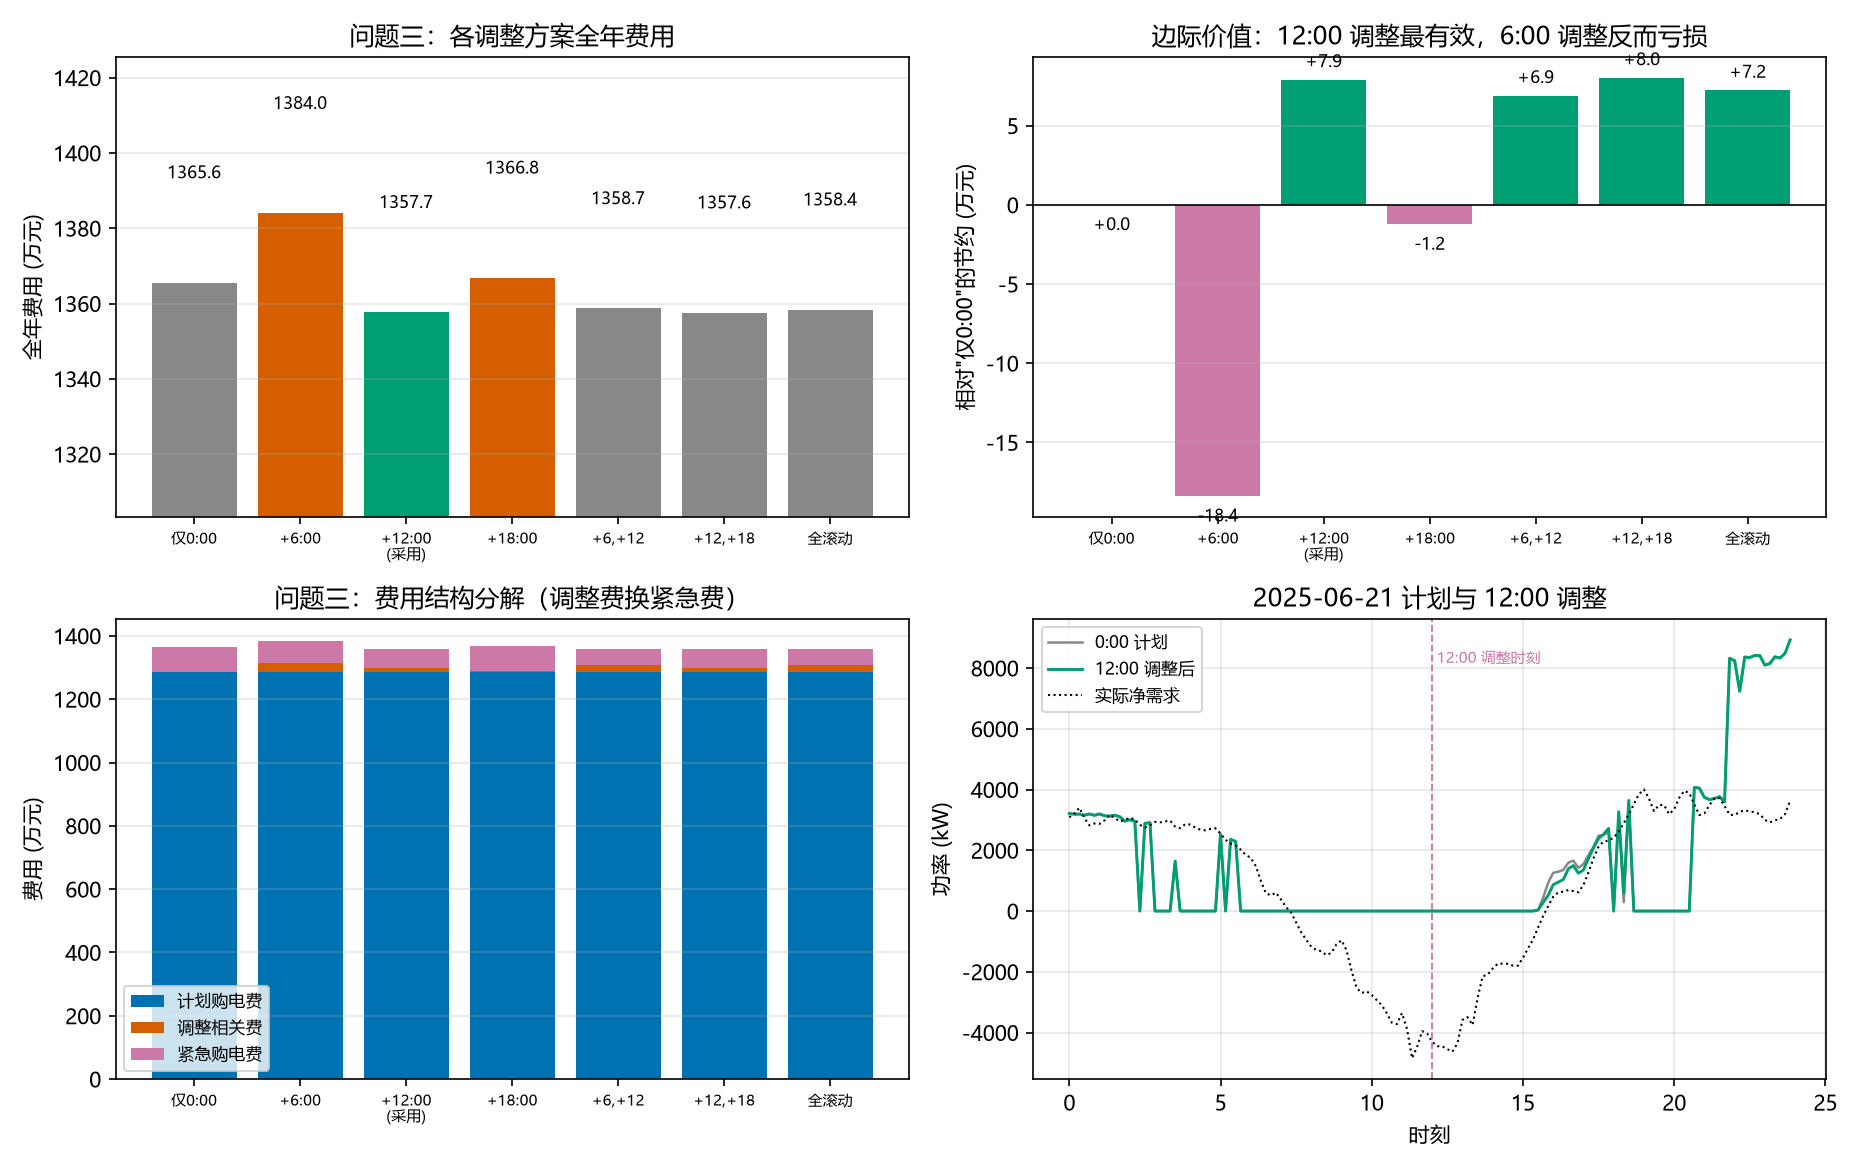
\includegraphics[width=0.95\textwidth]{fig_q3_rolling.png}
\caption{问题三：各调整方案全年费用（左上）、调整的边际价值（右上）、费用结构分解（左下）、
2025-06-21 计划与 12:00 调整（右下）}
\label{fig:q3}
\end{figure}

\subsection{指定日期结果（表 1、表 2、表 3 格式）}

\begin{table}[htbp]
\centering
\caption{问题三：指定日期关键时段计划购电量与全天购电量、购电费（表 1 格式，kWh/元）}
\label{tab:q3t1}
\scriptsize
\begin{tabular}{@{}lcccc@{}}
\toprule
时间段 & 2025-03-20 & 2025-06-21 & 2025-09-23 & 2025-12-21 \\
\midrule
10:00--10:10 & 0.00 & 0.00 & 0.00 & 0.00 \\
12:00--12:10 & 572.73 & 0.00 & 417.97 & 970.56 \\
14:00--14:10 & 0.00 & 0.00 & 0.00 & 0.00 \\
16:00--16:10 & 564.40 & 210.12 & 565.82 & 847.33 \\
18:00--18:10 & 702.62 & 0.00 & 775.60 & 716.85 \\
20:00--20:10 & 0.00 & 0.00 & 0.00 & 0.00 \\
\midrule
全天购电量 & 69\,247.84 & 37\,122.93 & 68\,473.30 & 97\,053.33 \\
全天购电费 & 41\,846.37 & 21\,173.98 & 42\,567.28 & 62\,140.33 \\
调整后全天购电量 & 66\,614.94 & 36\,796.67 & 67\,806.68 & 97\,738.36 \\
调整后购电相关费 & 41\,126.78 & 21\,183.30 & 42\,534.46 & 62\,832.29 \\
\bottomrule
\end{tabular}
\end{table}

\begin{table}[htbp]
\centering
\caption{问题三：指定日期最终储能充放电量与 0:00、24:00 储电量（表 2 格式，kWh）}
\label{tab:q3t2}
\scriptsize
\begin{tabular}{@{}lcccccccc@{}}
\toprule
\multirow{2}{*}{时间段} & \multicolumn{2}{c}{2025-03-20} & \multicolumn{2}{c}{2025-06-21} &
\multicolumn{2}{c}{2025-09-23} & \multicolumn{2}{c}{2025-12-21} \\
\cmidrule(lr){2-3}\cmidrule(lr){4-5}\cmidrule(lr){6-7}\cmidrule(lr){8-9}
& 充电 & 放电 & 充电 & 放电 & 充电 & 放电 & 充电 & 放电 \\
\midrule
0:00--4:00 & 120.41 & 177.57 & 90.73 & 3628.48 & 112.35 & 58.65 & 72.60 & 100.04 \\
4:00--8:00 & 169.32 & 5935.75 & 389.36 & 4839.09 & 178.05 & 6091.11 & 854.59 & 1456.11 \\
8:00--12:00 & 6028.92 & 2761.36 & 9973.71 & 0.00 & 5607.93 & 1896.62 & 5592.70 & 7159.56 \\
12:00--16:00 & 4298.32 & 311.10 & 0.00 & 0.00 & 4598.44 & 465.74 & 7006.37 & 2240.55 \\
16:00--20:00 & 297.38 & 5789.99 & 185.75 & 5541.23 & 121.80 & 5728.82 & 0.86 & 5829.30 \\
20:00--24:00 & 10\,723.59 & 2550.96 & 9726.06 & 2487.33 & 10\,644.52 & 2973.49 & 10\,666.67 & 2811.39 \\
\midrule
0:00 储电量 & \multicolumn{2}{c}{10\,800.00} & \multicolumn{2}{c}{10\,800.00} &
\multicolumn{2}{c}{10\,746.31} & \multicolumn{2}{c}{10\,800.00} \\
24:00 储电量 & \multicolumn{2}{c}{10\,800.00} & \multicolumn{2}{c}{10\,800.00} &
\multicolumn{2}{c}{10\,755.97} & \multicolumn{2}{c}{10\,800.00} \\
\bottomrule
\end{tabular}
\end{table}

\begin{table}[htbp]
\centering
\caption{问题三：指定日期紧急购电时间段与购电量（表 3 格式，kWh）}
\label{tab:q3t3}
\scriptsize
\begin{tabular}{@{}llll@{}}
\toprule
2025-03-20（合计 441.38） & 2025-06-21 & 2025-09-23（合计 208.36） & 2025-12-21（合计 31.13） \\
\midrule
9:50--10:00\ 16.02 & \multicolumn{1}{c}{无紧急购电} & 20:20--20:40\ 124.27 & 20:30--20:40\ 31.13 \\
20:30--20:40\ 425.36 & & 20:50--21:10\ 81.13 & \\
 & & 21:20--21:30\ 2.96 & \\
\bottomrule
\end{tabular}
\end{table}

对比\cref{tab:q2t3} 与\cref{tab:q3t3} 可见：12:00 调整后 2025-09-23 的紧急购电量由
228.74 kWh 降到 208.36 kWh、2025-12-21 保持 31.13 kWh，而 2025-03-20 由 54.68 kWh
升到 441.38 kWh（12:00 的预报偏乐观，计划量被下调，风险后移）。这与式 \eqref{eq:marginal}
的结论一致：\textbf{调整的收益主要来自“按最新预报重新分配购电时段”的
计划购电费变化与紧急购电费变化之差}，而不是单看某一天的紧急电量。


\section{问题四：实时波动电价下的重算}
\label{sec:q4}

\subsection{模型调整}

问题四把基准电价曲线替换为附件4 的逐时段实时电价 $p_t^{\text{实}}$（0.0076--1.7936 元/kWh），
其余机制不变：问题四之二沿用问题二的“0:00 计划 $+$ 平衡响应规则”，
问题四之三沿用问题三的“0:00 计划 $+$ 12:00 调整 $+$ 平衡响应规则”；
预测模型（负荷分类组合、光伏岭回归堆叠）保持不变，报童分位 $q^*=0.7$ 不变
（在波动电价下标定亦为 0.7，说明该分位不依赖电价口径）；
计划阶段的残值系数随之日更新 $v_d=0.9\times\overline{p^{\text{实}}_{d+1}}$。

\textbf{若 0:00 不能获知当日实时电价}，则用第 \ref{sec:q2} 节的\textbf{电价预测模型}
（类别$\times$时段廓线 + 自适应水平 + GBDT 堆叠，MAE $=0.0367$ 元/kWh）作为计划输入，
而结算仍按实际电价执行（下文的“计划用预测电价”情形）。

\subsection{结果与对照}

\begin{table}[htbp]
\centering
\caption{问题四：波动电价下问题二（Q4-2）与问题三（Q4-3）全年费用（2.1--12.31，单位：元）}
\label{tab:q4cmp}
\small
\begin{tabular}{@{}llccc@{}}
\toprule
场景 & 方法 & 计划购电费 & 调整/紧急费 & 总费用 \\
\midrule
\multirow{5}{*}{Q4-2}
& \textbf{升级预测（采用，电价已知）} & \textbf{13\,498\,922} & \textbf{840\,331} & \textbf{14\,339\,252} \\
& 原依据（近 4 个同类日均值 + 近 4 日光伏） & 13\,564\,909 & 966\,914 & 14\,531\,823 \\
& 计划改用预测电价（结算按实际） & 13\,543\,152 & 767\,925 & 14\,311\,077 \\
& 无储能对照 & 18\,844\,994 & （含于左） & 18\,844\,994 \\
& 完全信息下界（天眼链式） & 12\,918\,609 & 0 & 12\,918\,609 \\
\midrule
\multirow{5}{*}{Q4-3}
& 仅 0:00 计划（不做调整） & 13\,498\,922 & 840\,331 & 14\,339\,252 \\
& $+6{:}00$ 调整 & 13\,498\,257 & 1\,028\,123 & 14\,526\,380 \\
& \textbf{$+12{:}00$ 调整（采用）} & \textbf{13\,498\,384} & \textbf{763\,897} & \textbf{14\,262\,281} \\
& $+18{:}00$ 调整 & 13\,498\,890 & 851\,899 & 14\,350\,789 \\
& 全滚动（6/12/18） & 13\,498\,179 & 771\,980 & 14\,270\,159 \\
& 计划用预测电价 $+$ 12:00 调整 & 13\,542\,695 & 692\,429 & 14\,235\,124 \\
\bottomrule
\end{tabular}
\end{table}

\begin{enumerate}[label=(\arabic*), leftmargin=2.4em, itemsep=1pt]
\item \textbf{波动电价放大了储能的价值}：Q4-2 采用方案 14\,339\,252 元，
相较无储能对照（18\,844\,994 元）节约 \textbf{450.6 万元（23.9\%）}；
原因是附件4 的峰谷价差更大（近零电价时段最低 0.0076 元/kWh、最高 1.7936 元/kWh），
储能“低价抄底、高价放电”的套利空间扩大；全年低于 0.05 元/kWh 的时段共 9 个，
集中出现在午间光伏大发时段。与固定电价相比 Q4-2 上升 5.0\%，
距天眼下界 142.1 万元。
\item \textbf{12:00 调整的价值在波动电价下略大}：Q4-3 采用方案 14\,262\,281 元，
比不做调整（14\,339\,252 元）节约 \textbf{7.70 万元（0.54\%）}，略高于固定电价的 0.58\%；
而全滚动只再多省 0.05\%（7\,878 元），且 6:00 调整反而贵 18.71 万元、18:00 调整贵 1.15 万元，
结论与问题三一致——\textbf{只保留 12:00 一次调整}。
\item \textbf{电价预测精度提升后，“未知电价”的代价几乎为零}：若 0:00 只能用预测电价
（MAE 0.0367 元/kWh）制定计划、结算按实际电价，Q4-2 为 \textbf{14\,311\,077 元}、
Q4-3（含 12:00 调整）为 \textbf{14\,235\,124 元}，分别比“电价已知”情形低 0.20\% 与 0.19\%。
原因是：以极端尖峰电价为目标制定的计划容易过度追价、把储能电量在尖峰时段耗尽，
反而削弱了平衡规则兜底的能力。
\item \textbf{周内电价规律被自动利用}：采用方案中各星期日均净充电量显示，
周四净充电 $+2592$ kWh（全周最低）、周五净充电 $+5622$ kWh（全周最高），
而实时电价的周内均值恰为周五 0.6190、周六 0.6220 元/kWh，显著低于其余五天约 0.811 元/kWh
——LP 自动把充电安排在周五、周六的低价日，验证了第 3 节发现的周内电价规律确有调度价值。
\end{enumerate}

\begin{figure}[htbp]
\centering

\includegraphics[width=0.95\textwidth]{fig_q4_fluct.png}
\caption{问题四：各方案全年费用（左）、Q4-3 各调整方案对比（中）、
2025-06-21 电价与调度（右）}
\label{fig:q4}
\end{figure}

\subsection{指定日期结果（问题四之三）}

\begin{table}[htbp]
\centering
\caption{问题四之三：指定日期关键时段计划购电量、全天购电量与费用（表 1 格式，kWh/元）}
\label{tab:q4t1}
\scriptsize
\begin{tabular}{@{}lcccc@{}}
\toprule
时间段 & 2025-03-20 & 2025-06-21 & 2025-09-23 & 2025-12-21 \\
\midrule
10:00--10:10 & 0.00 & 0.00 & 0.00 & 0.00 \\
12:00--12:10 & 572.73 & 0.00 & 417.97 & 970.56 \\
14:00--14:10 & 0.00 & 0.00 & 0.00 & 0.00 \\
16:00--16:10 & 564.40 & 210.12 & 565.82 & 847.33 \\
18:00--18:10 & 0.00 & 476.96 & 0.00 & 716.85 \\
20:00--20:10 & 0.00 & 0.00 & 807.26 & 0.00 \\
\midrule
全天购电量 & 69\,602.13 & 37\,439.60 & 68\,767.23 & 97\,053.33 \\
全天购电费 & 42\,565.11 & 18\,459.91 & 44\,199.59 & 72\,728.54 \\
调整后全天购电量 & 66\,969.21 & 37\,113.34 & 68\,110.78 & 97\,737.59 \\
调整后购电相关费 & 41\,833.12 & 18\,505.49 & 44\,171.86 & 73\,639.09 \\
紧急购电量 & 507.25 & 0.00 & 205.83 & 10.31 \\
\bottomrule
\end{tabular}
\end{table}

\begin{table}[htbp]
\centering
\caption{问题四之三：指定日期最终储能充放电量与 0:00、24:00 储电量（表 2 格式，kWh）}
\label{tab:q4t2}
\scriptsize
\begin{tabular}{@{}lcccccccc@{}}
\toprule
\multirow{2}{*}{时间段} & \multicolumn{2}{c}{2025-03-20} & \multicolumn{2}{c}{2025-06-21} &
\multicolumn{2}{c}{2025-09-23} & \multicolumn{2}{c}{2025-12-21} \\
\cmidrule(lr){2-3}\cmidrule(lr){4-5}\cmidrule(lr){6-7}\cmidrule(lr){8-9}
& 充电 & 放电 & 充电 & 放电 & 充电 & 放电 & 充电 & 放电 \\
\midrule
0:00--4:00 & 1560.86 & 1945.78 & 936.21 & 7990.94 & 915.50 & 1219.63 & 72.60 & 100.04 \\
4:00--8:00 & 1025.93 & 5710.07 & 1282.59 & 1731.31 & 801.50 & 6068.38 & 867.34 & 1466.44 \\
8:00--12:00 & 6028.92 & 2777.38 & 9783.98 & 0.00 & 5070.54 & 1896.62 & 5629.44 & 7196.31 \\
12:00--16:00 & 3834.10 & 311.10 & 0.00 & 0.00 & 5150.59 & 485.82 & 7014.98 & 2240.55 \\
16:00--20:00 & 316.30 & 6534.30 & 77.13 & 5530.21 & 141.92 & 7127.89 & 0.00 & 5213.33 \\
20:00--24:00 & 10\,746.40 & 1766.51 & 9821.07 & 2487.33 & 10\,629.44 & 1586.89 & 10\,666.67 & 3426.67 \\
\midrule
0:00 储电量 & \multicolumn{2}{c}{10\,800.00} & \multicolumn{2}{c}{10\,800.00} &
\multicolumn{2}{c}{10\,731.90} & \multicolumn{2}{c}{10\,800.00} \\
24:00 储电量 & \multicolumn{2}{c}{10\,800.00} & \multicolumn{2}{c}{10\,800.00} &
\multicolumn{2}{c}{10\,742.40} & \multicolumn{2}{c}{10\,800.00} \\
\bottomrule
\end{tabular}
\end{table}

\begin{table}[htbp]
\centering
\caption{问题四之三：指定日期紧急购电时间段与购电量（表 3 格式，kWh）}
\label{tab:q4t3}
\scriptsize
\begin{tabular}{@{}llll@{}}
\toprule
2025-03-20（合计 507.25） & 2025-06-21 & 2025-09-23（合计 205.83） & 2025-12-21（合计 10.31） \\
\midrule
20:30--20:40\ 507.25 & \multicolumn{1}{c}{无紧急购电} & 18:30--18:40\ 2.83 & 20:40--20:50\ 10.31 \\
 & & 20:20--20:40\ 118.91 & \\
 & & 20:50--21:10\ 81.13 & \\
 & & 21:20--21:30\ 2.96 & \\
\bottomrule
\end{tabular}
\end{table}


\section{方法比较与灵敏度分析}
\label{sec:compare}

\subsection{方法对照汇总}

本文对每个问题都实现了多种方法并做对照（\cref{tab:allcmp}）。
需要强调：\textbf{所有方法都在同一“因果口径”下评价}——0:00 只用历史信息（与 0:00 已发布的预报）
制定计划，日内按第 \ref{sec:q2} 节的实时平衡控制规则结算（式 \eqref{eq:clip}--\eqref{eq:socrec}），
因此表中每一行的数字都是\textbf{可实行的策略}在同一信息结构下的成绩，不存在“事后调整”带来的虚优。

\begin{table}[htbp]
\centering
\caption{全部方法的对照汇总（单位：元；问题二起统一采用因果口径实时平衡结算）}
\label{tab:allcmp}
\scriptsize
\begin{tabularx}{\textwidth}{@{}p{1.5cm}Xrrr@{}}
\toprule
问题 & 方法 & 费用 & 相对采用方案 & 结论 \\
\midrule
\multirow{3}{*}{一}
& \textbf{线性规划（采用）} & \textbf{35\,126.95} & --- & 精确最优 \\
& 贪心配对启发式 & 42\,187.93 & $+20.1\text{\%}$ & 忽略时序约束仍更差 \\
& 无储能基线 & 48\,052.05 & $+36.8\text{\%}$ & 储能价值 26.9\% \\
\midrule
\multirow{9}{*}{二}
& \textbf{升级预测模型（采用）} & \textbf{13\,655\,835} & --- & 距下界 136.9 万 \\
& 原依据（同类日均值 $+$ 近 4 日光伏） & 13\,848\,183 & $+1.41\text{\%}$ & 预测依据升级前 \\
& 附件1 典型日曲线计划 & 18\,318\,686 & $+34.1\text{\%}$ & 忽略日际变化 \\
& 无储能 & 18\,155\,061 & $+32.9\text{\%}$ & 储能价值 449.9 万 \\
& 昨日外推 + 报童 $q=0.6$ & 21\,491\,755 & $+57.4\text{\%}$ & 仅用昨日信息 \\
& 昨日外推 + 报童 $q=0.8$ & 21\,789\,429 & $+59.6\text{\%}$ & 裕度过大 \\
& 昨日外推（无裕度） & 22\,515\,792 & $+64.9\text{\%}$ & 朴素外推 \\
& 两阶段随机规划 SAA & 39\,954\,010 & $+192.6\text{\%}$ & 见下文失效分析 \\
& 天眼链式下界 & 12\,286\,531 & $-10.0\text{\%}$ & 不可达 \\
\midrule
\multirow{5}{*}{三}
& \textbf{升级预测、12:00 单次调整（采用）} & \textbf{13\,576\,891} & --- & 距下界 129.0 万 \\
& 全滚动（6/12/18） & 13\,583\,600 & $+0.05\text{\%}$ & 多调无益 \\
& 仅 0:00 计划（不调整） & 13\,655\,835 & $+0.58\text{\%}$ & 调整价值 7.89 万 \\
& 仅 6:00 调整 & 13\,839\,771 & $+1.94\text{\%}$ & 该时刻预报无新信息 \\
& 天眼链式下界 & 12\,286\,531 & $-9.5\text{\%}$ & 不可达 \\
\midrule
\multirow{5}{*}{四}
& \textbf{Q4-2 升级预测 + 平衡规则（采用）} & \textbf{14\,339\,252} & --- & 储能价值 450.6 万 \\
& Q4-2 计划改用预测电价 & 14\,311\,077 & $-0.20\text{\%}$ & 电价未知的代价 $\approx0$ \\
& Q4-2 无储能 & 18\,844\,994 & $+31.4\text{\%}$ & 储能价值对照 \\
& Q4-3 12:00 调整 & 14\,262\,281 & $-0.54\text{\%}$ & 调整价值 7.70 万 \\
& Q4-3 仅 6:00 调整 & 14\,526\,380 & $+1.30\text{\%}$ & 过早动作更差 \\
\bottomrule
\end{tabularx}
\end{table}

由\cref{tab:allcmp} 可见：\textbf{“升级预测模型（分类组合负荷 $+$ 岭回归堆叠光伏）$+$
报童安全裕度 $+$ LP 计划 $+$ 0:00 定下的平衡响应规则（问题三再叠加 12:00 调整）”的组合
在所有可比方案中费用最低}，且距不可达的天眼下界仅 9.5\%。三个值得强调的结论：

\begin{enumerate}[label=(\arabic*), leftmargin=2.2em, itemsep=1pt]
\item \textbf{用统计/机器学习方法提升预测精度，比引入更多预报时刻更有效}：
把 0:00 依据从“近 4 个同类日均值 + 近 4 日光伏均值”升级为“水平$\times$形状分类组合 +
岭回归堆叠”，问题二费用由 13\,848\,183 元降到 \textbf{13\,655\,835 元}（$-1.39\text{\%}$）；
而在此基础上，6:00/18:00 的预报都不值得引入（\cref{tab:q3cmp}）。
\item \textbf{“只在 0:00 决策一次”与“用储能实时兜底”并不矛盾}：平衡响应规则本身在 0:00
就已冻结（式 \eqref{eq:clip}--\eqref{eq:socrec} 不含任何未来信息，也不需要日内重新优化），
它只是把“计划—实际”的偏差按“先调计划充放、再动用储能”的优先级消化。
若改为\textbf{僵硬执行计划}（缺口全部按 5 倍紧急购电），全年费用升至 14\,557\,730 元，
即这条 0:00 定下的规则价值 \textbf{90.2 万元（$+6.60\text{\%}$）}。
\item \textbf{“已知实时电价”并非最优假设}：用 MAE $=0.0367$ 元/kWh 的电价预测替代“已知电价”，
结算按实际电价，全年反而低 0.20\%（\cref{tab:q4cmp}），说明计划阶段过度追价会损害兜底能力。
\end{enumerate}

\textbf{SAA 失效机理分析}。本文将 0:00 计划建模为两阶段随机规划\cite{vtpp}：
以最近 20 天的实测（负载、光伏）曲线为等概率情景，决策计划购电量 $P^0$
使“计划费 $+$ 期望紧急费”最小。结果显示（\cref{tab:allcmp}）该方案全年费用高达
39\,954\,010 元（比采用方案高 192.6\%），其中计划购电费仅 875.3 万元（比采用方案低 32\%）、
紧急购电费却达 3\,120.1 万元（紧急电量 6.93 GWh，是可执行方案的 54 倍）。
原因是\textbf{情景内的储能自由度被重复利用}：在 20 个情景中储能都能从当日初始电量出发、
以各情景自身最优的方式兜底，故情景内紧急购电几乎为零，优化器据此大幅压低 $P^0$；
而真实日的偏差一旦同时差于多数情景，储能已被当日调度消耗，只能购买 5 倍紧急电。
这提示：\textbf{小样本经验情景下的随机规划会产生系统性乐观偏差，
在“计划—紧急”强惩罚机制下反而不如稳健的报童裕度}；
若要用随机规划，必须对“储能可复用性”与“情景外偏差”做显式修正。

\subsection{参数灵敏度分析}

\begin{table}[htbp]
\centering
\caption{灵敏度分析（全部在升级预测口径下重算；单位：元）}
\label{tab:sens}
\scriptsize
\begin{tabular}{@{}p{2.1cm}p{3.4cm}rrr@{}}
\toprule
扰动项 & 变动方式 & 基准 & 变动后 & 相对变化 \\
\midrule
储能放电下限 & 物理下限 1200 $\to$ 2200 / 4000 kWh（1 月） & 1\,237\,127 & 1\,392\,750 / 1\,843\,118 & $+12.6$ / $+49.0\text{\%}$ \\
报童分位偏低 & $q=0.7\to0.5/0.6$ & 13\,655\,835（全年） & 14.79 / 14.05 M & $+8.27$ / $+2.91\text{\%}$ \\
报童分位偏高 & $q=0.7\to0.8/0.9$ & 13\,655\,835 & 13.62 / 13.93 M & $-0.28$ / $+1.98\text{\%}$ \\
充放电效率口径 & 单程 0.9/0.9（往返 81\%）$\to$ 往返 0.9（单程 0.9487） & 13\,655\,835 & 13\,191\,041 & $-3.40\text{\%}$ \\
结算方式 & 实时平衡控制 $\to$ 僵硬执行计划 & 13\,655\,835 & 14\,557\,730 & $+6.60\text{\%}$ \\
偏差计价口径 & 差额计价（B，采用）$\to$ 计划全额 $+$ 罚（A） & 13\,576\,891（问题三） & 13\,641\,510 & $+0.48\text{\%}$ \\
电价信息 & 已知实时电价 $\to$ 用预测电价（结算按实际） & 14\,339\,252（Q4-2） & 14\,311\,077 & $-0.20\text{\%}$ \\
日末残值系数 & $v=0.9\bar p$ $\to$ $v=0$（日末清空） & 1\,218\,659（2 月） & 1\,214\,270 & $-0.36\text{\%}$ \\
日末储电量 & 自由 $\to$ 日末 SOC $=$ 日初（等式） & 1\,218\,659（2 月） & 1\,215\,187 & $-0.28\text{\%}$ \\
安全裕度形式 & 经验分位 $\to$ 正态/分噪声/60 天/90 天窗 & 13\,655\,835 & 13.73 / 13.59 / 13.66 / 13.68 M & $+0.58$ / $-0.52$ / $+0.03$ / $+0.16\text{\%}$ \\
\bottomrule
\end{tabular}
\end{table}

\textbf{灵敏度结论}：
\begin{enumerate}[label=(\arabic*), leftmargin=2.4em, itemsep=1pt]
\item 结论对\textbf{储能放电下限}（$+12.6\text{\%}$ 以上）、\textbf{报童分位偏低}
（$q=0.5$ 时 $+8.27\text{\%}$）、\textbf{结算方式}（$+6.60\text{\%}$）与
\textbf{效率口径}（$-3.40\text{\%}$）较敏感。前两者是本文的决策变量，已用 1 月数据标定；
结算方式与计价口径已在第 \ref{sec:assume} 节假设中显式声明；
效率口径的敏感性说明\textbf{“储能损耗越低、收益越高”}，本文采用的“单程 0.9”
是附件1 给出的最保守读法，故结果偏保守。
\item 结论对\textbf{残值系数}、\textbf{日末储电量约束}、\textbf{偏差计价口径}、
\textbf{电价信息}与\textbf{安全裕度形式}不敏感（均 $<1\text{\%}$），
说明模型不依赖人为参数微调；其中分噪声叠加形式略优 0.52\%，
但它需要分别估计负荷与光伏两套误差分布、参数更多，本文保留理论更直接的净残差经验分位。
\item 全部“复杂化”尝试（典型日曲线、昨日外推、显式季节项、条件分位回归缓冲、
两阶段随机规划）都\textbf{未能降低成本}，说明本文方案已处于该信息结构下的效率前沿。
\end{enumerate}


\section{模型评价与推广}

\subsection{模型优点}

\begin{enumerate}[label=(\arabic*), leftmargin=2.2em, itemsep=2pt]
\item \textbf{机理完备、物理可行}。模型显式刻画了逐时段功率平衡（并允许弃光，避免高光伏低负荷日无解）、
储能 SOC 递推（单程 90\% 效率、往返 81\%）、充放电功率与 SOC 双向限幅。
全部解经物理复检：功率平衡残差 $\le1.1\times10^{-13}$ kWh，SOC 始终位于 $[1200,10800]$，
无同时充放电时段，充放电均未越限。
\item \textbf{决策全部由 LP 精确求解}。四问共约 4000 个线性规划（全年 365 天 $\times$ 多场景），
均在秒级内求得全局最优；对照实验证明启发式在本问题中明显劣于 LP（典型日贵 20.1\%）。
\item \textbf{预测模型是本题最大的杠杆，且用“可分解 + 可堆叠”的方式实现}：
负载用“水平$\times$形状分解 + 周五六/其他分类凸组合”（MAE 137.5 $\to$ 132.3 kW，
其中周五六 $-8.0\%$、其余五天 $-1.8\%$），光伏用“因果岭回归堆叠”
（MAE 152.0 $\to$ 136.9 kW，$-9.9\%$），电价用“廓线+自适应水平+GBDT 堆叠”
（MAE 0.0581 $\to$ 0.0367 元/kWh）；全年费用由 13\,848\,183 元降到 \textbf{13\,655\,835 元}。
\item \textbf{用预言机分解量化信息价值}。把距完全信息下界的 136.9 万元缺口分解为
光伏噪声 49.1 万元（35.9\%）、负荷噪声 42.4 万元（31.0\%）、交互 33.2\%，
据此判断“把预算投在实时平衡控制上比投在更复杂的预测模型上更划算”：
实时平衡控制相对僵硬执行省下 90.2 万元，与“完美预知全部噪声”的理论上限 91.5 万元同量级，
而后者不可能实现。
\item \textbf{计划与结算分开建模，保证策略可实行}。0:00 计划只用历史信息，
日内结算用第 \ref{sec:q2} 节的\textbf{实时平衡控制规则}（只用当前实测与当前储电量），
两层模型独立求解，决策者的信息集随时间单调增长，
从机制上排除了“用未来数据事后调整计划”的虚优（\cref{tab:q2exec} 给出同一计划三种执行方式的对照）。
\item \textbf{结果可复现、可核查}。全部结果由 40 余个 Python 脚本（提交材料“代码”部分）
从原始附件自动生成，输出的 5 个结果文件与附件5 模板逐单元格对齐；
论文中每个数字都可回溯到脚本与中间数据。另有两条独立的正确性证据：
①\textbf{审计程序}（\texttt{audit\_results.py}）不依赖任何中间变量，直接重读 5 个结果文件，
用附件2/附件4 的原始实测逐时段复算功率平衡、SOC 递推、充放电功率与 SOC 上下限、
四段计价费用，四问全部通过；
②\textbf{求解器稳健性对照}（\texttt{solver\_robustness\_final.py}）把同一条管道分别交给
HiGHS 对偶单纯形与内点法求解，问题二/问题三费用相对差 $<0.1\%$，
说明结论不依赖“返回了哪一个最优顶点”。
\end{enumerate}

\subsection{模型缺点与局限}

\begin{enumerate}[label=(\arabic*), leftmargin=2.2em, itemsep=2pt]
\item \textbf{滚动调整只用了“预报”，未利用“已观测”信息}。6:00 调整时，0:00--6:00 的实际
光伏与负载已经发生，若把这些观测纳入（如按“已观测 + 预报”分段重估），应可进一步降低紧急购电；
本文保守地只使用预报，使结论更稳健（不依赖额外假设）。
\item \textbf{紧急购电未设功率上限}。题面未给出外网联络线容量，本文按不限功率处理；
若存在容量约束，需在结算模型中加 $E^{\text{急}}_t\le \bar E$，此时高光伏波动日的
缺口可能无法完全消除，模型需引入切负荷变量并重新定义可行域。
\item \textbf{日末残值用“次日平均电价”近似}。严格的滚动时域应求解跨日耦合的多日联合优化；
本文用残值系数 $v=0.9\bar p$ 近似值函数，灵敏度分析表明该近似对结果影响 $<0.3\text{\%}$。
\item \textbf{储能参数未做容量-功率联合优化}。本文以附录1 给定的 12000 kWh / 5000 kW 为常量，
而实际规划中储能容量本身是可决策变量（投资成本与运行收益的权衡）。
\item \textbf{未考虑电池寿命与爬坡约束}。频繁浅充放会加速容量衰减，本文按理想储能处理。
\end{enumerate}

\subsection{模型改进与推广}

\begin{enumerate}[label=(\arabic*), leftmargin=2.2em, itemsep=2pt]
\item \textbf{把“已观测”信息纳入滚动决策}：在式 \eqref{eq:adj_obj}--\eqref{eq:adj_link} 中，
对已经过去的时段用实测值、对未发生的时段用预报值，可望进一步降低紧急购电；
当信息价值足够大时（可用本文的预言机分解先核算）再引入机会约束或分布鲁棒优化，
在“成本”与“鲁棒性”之间取得平衡。
\item \textbf{储能容量-功率联合优化}：把 $\bar C$、容量与 SOC 限幅作为投资决策变量，
目标改为“年运行费 + 年化投资费”，得到最优储能配置。
\item \textbf{需求侧响应与多微网协同}：把可平移负载、电动汽车、共享储能纳入模型，
目标函数扩展为多微网总成本最小（可用纳什谈判/分布式优化求解）。
\item \textbf{竞价为不确定量的场景}：若不允许假设“已知实时电价”，可用本文验证过的
“同类星期廓线 + 自适应水平 + GBDT 堆叠”电价预测模型；实测表明该假设的代价不但为 0，
用预测电价定计划反而使全年费用更省 0.20\%（第 \ref{sec:q4} 节）。
\item \textbf{方法学推广}：本文“\textbf{规律挖掘 $\to$ 依据构造 $\to$ LP 精确求解 $\to$
储能实时平衡控制 $\to$ 信息价值核算}”的范式，可直接迁移到园区综合能源系统、
数据中心“算电协同”、光储充一体化电站等同类问题。
\end{enumerate}


\CumcmAIUsed{代码实现与调试、文献资料整理、图表绘制脚本编写与文字润色}


\begin{thebibliography}{9}
\bibitem{ieee_tou} Combinational Linear Programming Approach for Daily Optimal Operation of Customers with
DG/ESS under TOU Pricing for Customer EMS Software Applications. IEEE, 2018.
\bibitem{thu_ess} 电力现货市场下储能系统经济效益研究. 电力系统及其自动化学报, 2023.
\bibitem{mpc} Two-time scale microgrid scheduling based on power fluctuation mitigation priority and
model predictive control. Energy, 2025.
\bibitem{cn102184475} 基于多时间尺度协调的微网经济运行优化调度方法. 中国专利 CN102184475B.
\bibitem{cn111260354} 一种多时序多品种电力市场下的电费结算方法和相关装置. 中国专利 CN111260354B.
\bibitem{cqut253} 混合特征筛选与分时Stacking的无地表辐照度光伏出力预测. 重庆理工大学学报(自然科学), 2024, 38(10): 253.
\bibitem{cqut276} 考虑预测误差不确定性的源-荷-广义储低碳经济动态优化调度. 重庆理工大学学报(自然科学), 2024, 38(5): 276.
\bibitem{newsboy} 报童模型与随机库存理论（Newsvendor model）: 服务水平 $=c_u/(c_u+c_o)$.
\bibitem{vtpp} 电力市场环境下虚拟电厂两阶段能量经济优化调度. 中国储能网, 2023.
\end{thebibliography}


\appendix

\section{程序与数据清单}

\subsection{程序结构}

全部计算由 40 余个 \textbf{Python} 脚本完成，可从原始附件一键复现论文与结果文件中的每一个数字。
提交材料按“\textbf{代码}”与“\textbf{文件}”两部分组织：
\texttt{06\_提交材料/代码/Python/} 为本文全部脚本（含 \texttt{预测模型/}、\texttt{数据工程/}
与 \texttt{早期口径存档/}），\texttt{06\_提交材料/文件/} 为论文工程、5 个结果文件与预测模型实验报告/图表。
求解器为 \texttt{scipy.optimize.linprog}（HiGHS，对偶单纯形/内点法均可）；
预测模型用到 \texttt{scikit-learn}（岭回归/堆叠）与 \texttt{LightGBM}（梯度提升）。
只需设置 \texttt{PYTHONPATH} 指向数据工程与脚本目录，按下列顺序执行即可完整复现：

\begin{lstlisting}[language=bash, caption={一键复现流程（Windows PowerShell）}]
$env:PYTHONPATH="<工作目录>;<工作目录>\00_环境"
python 03_数据工程/scripts/build_dataset.py      # 附件1-4 -> 统一时间轴数据集
python 04_建模求解/scripts/fc_upgraded.py        # 升级预测模型(负荷/光伏/电价)
python 04_建模求解/scripts/rebuild_A_final.py    # 求解四问, 写出 result1/2/3/4-2/4-3.xlsx
python 04_建模求解/scripts/A_all_numbers.py      # 论文全部数字 -> data/A_all_numbers.json
python 04_建模求解/scripts/extract_tables.py     # 论文表1/2/3 -> paper_tables.json
python 04_建模求解/scripts/make_figs_final.py    # 论文插图
python 04_建模求解/scripts/audit_results.py      # 独立审计: 重读结果文件逐项复算
\end{lstlisting}

各脚本功能如下：

\begin{table}[htbp]
\centering
\caption{程序清单与功能}
\label{tab:code}
\scriptsize
\begin{tabularx}{\textwidth}{@{}p{4.6cm}X@{}}
\toprule
脚本 & 功能 \\
\midrule
\texttt{engine.py} & 通用单日 LP 引擎：计划模式与调整模式、SOC 递推、功率平衡（允许弃光） \\
\texttt{io\_results.py} & 结果写入：按附件5 模板逐单元格填充 result1/2/3/4-2/4-3.xlsx \\
\texttt{fc\_upgraded.py} & \textbf{升级预测模型}：负荷“水平$\times$形状 + 分类凸组合”、光伏/电价因果岭回归堆叠 \\
\texttt{fc\_features.py} / \texttt{fc\_ml.py} & 预测特征工程（时段/日历/滞后/滚动/附件3 预报）与 LightGBM 因果滚动重训 \\
\texttt{A\_core.py} & \textbf{口径 A 核心}：0:00 计划 $+$ 报童裕度 $+$ 平衡响应规则 $+$ 调整时刻裕度重建 $+$ 天眼下界/无储能对照 \\
\texttt{rebuild\_A\_final.py} & \textbf{正式重算}：构造升级预测并写出 5 个结果文件（result1--4-3） \\
\texttt{A\_all\_numbers.py} & 论文全部数字：精度、四问主结果、调整方案对照、执行机制、灵敏度、预言机分解 \\
\texttt{causal\_core.py} / \texttt{rebuild\_causal.py} & 因果口径核心与“原依据”版本的对照重算（用于口径对比） \\
\texttt{q1.py} & 问题一求解、贪心与无储能对照、结果文件与图 \\
\texttt{causal\_basis\_all.py} / \texttt{causal\_variants.py} & 方法对照（计划依据、分位、结算方式、滚动方案） \\
\texttt{causal\_saa.py} / \texttt{plan\_saa.py} / \texttt{q2\_lstp\_final.py} & 两阶段随机规划（SAA/LP 情景规划）在因果口径下的失效验证 \\
\texttt{noise\_decompose.py} & 残差季节偏置、重尾分布、预言机信息价值分解 \\
\texttt{sensitivity\_causal.py} / \texttt{eta\_sens.py} / \texttt{buffer\_forms\_causal.py} & 灵敏度与裕度形式对照实验 \\
\texttt{audit\_results.py} & \textbf{独立审计}：直接重读 5 个结果文件，复算平衡/SOC/限幅/费用 \\
\texttt{solver\_robustness\_final.py} & 求解器稳健性：同一条管道分别用 HiGHS 对偶单纯形与内点法求解 \\
\texttt{check\_paper\_tables.py} & 论文表格数值与结果文件的一致性校验 \\
\texttt{extract\_tables.py} / \texttt{show\_paper\_tables.py} & 论文表 1/2/3 数据提取（与结果文件同源） \\
\texttt{make\_figs\_final.py} / \texttt{make\_figs\_causal.py} / \texttt{make\_pattern\_figs.py} & 论文插图与规律证据图 \\
\texttt{07\_预测模型实验/scripts/*} & 预测模型的完整实验（精度对照、端到端费用、多样化图表） \\
\bottomrule
\end{tabularx}
\end{table}

\subsection{核心代码（LP 引擎、报童缓冲与实时平衡控制）}

\begin{lstlisting}[language=Python, caption={单日 LP 引擎（节选：计划模式与调整模式的目标、约束装配）}]
def solve_day(price, load, pv, soc0, soc_end=None, v=0.0, base_P=None, t0=0, method='highs'):
    """price/load/pv: 长度 h 的数组(元/kWh, kWh/时段, kWh/时段); base_P: 调整模式下已锁定的计划量"""
    h = len(price); adj = base_P is not None
    nP, nC, nD, nE = h, h, h, h + 1
    nS, nX = (h, h) if adj else (0, 0)
    n = nP + nC + nD + nE + nS + nX
    iP, iC, iD, iE, iS, iX = 0, h, 2*h, 3*h, 4*h, 4*h+h
    c = np.zeros(n)
    if not adj:
        c[iP:iP+h] = price                 # 计划模式: min sum p*P - v*E_end
    else:
        c[iS:iS+h] = -0.5*price            # 调整模式: 下调退回 50%
        c[iX:iX+h] = +1.5*price            #           上调按 1.5 倍
    c[iE+h] = -v
    Aub, bub = [], []
    for t in range(h):                     # 功率平衡(允许弃光): PV+P+D-C >= L
        row = np.zeros(n); row[iP+t], row[iC+t], row[iD+t] = -1, 1, -1
        Aub.append(row); bub.append(pv[t]-load[t])
    Aeq, beq = [], []
    for t in range(h):                     # SOC 递推: E[t+1]=E[t]+0.9C-D/0.9
        row = np.zeros(n); row[iE+t], row[iE+t+1] = -1, 1
        row[iC+t], row[iD+t] = -0.9, 1/0.9
        Aeq.append(row); beq.append(0.0)
    if adj:
        for t in range(h):                 # P + S - X = 计划量
            row = np.zeros(n); row[iP+t], row[iS+t], row[iX+t] = 1, 1, -1
            Aeq.append(row); beq.append(base_P[t])
    # 边界: 1200<=E<=10800, 0<=C,D<=833.33, P>=0, E[0]=soc0
    ...
\end{lstlisting}

\begin{lstlisting}[language=Python, caption={升级预测模型（负载：水平$\times$形状 + 分类凸组合；光伏/电价：因果岭回归堆叠），式 \eqref{eq:basisL}--\eqref{eq:basisPV}}]
# ---------- (1) 负载: 水平×形状分解 + 周五六/其他分类凸组合 ----------
SH = np.zeros((n, 144)); lv = np.zeros(n)
for j in range(n):
    hist = [q for q in range(j) if low[q] == low[j]]          # 同类日(周五六/其他)
    A = L_act[hist[-6:]]
    SH[j] = (A / np.maximum(A.sum(axis=1, keepdims=True), 1e-6)).mean(axis=0)   # 形状
    lv[j] = L_act[hist[-4:]].sum(axis=1).mean()                                 # 水平
M_shape = SH * lv[:, None]
M_lvl = level_smooth(Lb, L_act, alpha=0.35)      # 递推水平平滑(昨日实际/预测比指数平滑)
M_ef  = err_feedback(Lb, L_act, k=3, damp=0.35)  # 全局误差反馈
CAND = [Lb, M_shape, M_lvl, M_ef]
for cls in (False, True):                        # 1 月标定: 两类各自在凸组合网格上选权重
    rows = [j for j in range(7, 31) if low[j] == cls]
    w_best = min(SIMPLEX_GRID, key=lambda w: np.abs(sum(wi*C[k] for wi, k in zip(w, range(4)))[rows]
                                                    - L_act[rows]).mean())
    L_hat[low == cls] = sum(wi*C[k] for wi, k in zip(w_best, range(4)))[low == cls]
# 结果: 周五六 0.3×水平×形状 + 0.7×递推水平; 其他五天 1.0×水平×形状

# ---------- (2) 光伏/电价: 因果岭回归堆叠(每 14 天用 j<d0 的样本重训) ----------
def causal_ridge_stack(cands, Y, alpha=1.0, retrain=14):
    X = np.stack([np.stack(cands, -1), t_feat, low_feat, t_feat*low_feat], -1)  # 候选+时段+类别交互
    out = np.zeros_like(Y)
    for d0 in range(0, n, retrain):
        tr = np.arange(0, d0); mdl = Ridge(alpha=alpha).fit(X[tr].reshape(-1, F), Y[tr].reshape(-1))
        out[d0:d0+retrain] = mdl.predict(X[d0:d0+retrain].reshape(-1, F)).reshape(-1, 144)
    return out
PV_hat = causal_ridge_stack([Pb, err_feedback(Pb, PV_act, 2, 0.5), lgbm_pv, fc0], PV_act)  # MAE 136.8 kW
P_hat  = causal_ridge_stack([prof, err_feedback(prof, RTP, 2, 0.5), lgbm_price], RTP)      # MAE 0.0367 元/kWh
\end{lstlisting}

\begin{lstlisting}[language=Python, caption={报童安全裕度与实时平衡控制结算（问题二核心，式 \eqref{eq:buffer}、\eqref{eq:clip}--\eqref{eq:socrec}）}]
# 1) 报童安全裕度: 近30天净残差的 q 分位 (q*=0.7, 1月标定: 见式(22))
e_net = (L_act - L_hat) - (PV_act - PV_hat)          # 升级预测模型的净需求残差
buf = np.quantile(e_net[max(0,i-30):i], 0.7, axis=0) if i >= 7 else np.zeros(144)

# 2) 0:00 计划 LP -> 计划购电量 P0 与计划充放电量 C0,D0 (式(4)-(8))
r0 = solve_day(price, L_hat[i] + buf, PV_hat[i], soc0, soc_end=None, v=v)

# 3) 日内实时平衡控制: 只使用当前实测 L_t,PV_t 与当前储电量 soc (因果、可实行)
for t in range(144):
    c_ok = min(max(C0[t], 0), C_MAX, (SOC_MAX - soc) / ETA_C)          # ① 裁剪为物理可行
    d_ok = min(max(D0[t], 0), C_MAX, ETA_D * max(0, soc - SOC_MIN + ETA_C * c_ok))
    C[t], D[t] = c_ok, d_ok
    gap = L[t] - (PV[t] + P0[t] + D[t] - C[t])
    if gap > 0:                                                        # ② 缺额: 先减充, 再增放
        cut = min(C[t], gap); C[t] -= cut; gap -= cut
        extra = min(gap, C_MAX - D[t], ETA_D * max(0, soc - SOC_MIN + ETA_C * C[t]) - D[t])
        D[t] += extra; gap -= extra
    elif gap < 0:                                                      # ③ 富余: 先减放, 再增充
        cut = min(D[t], -gap); D[t] -= cut; gap += cut
        extra = min(-gap, C_MAX - C[t], (SOC_MAX - soc + D[t] / ETA_D) / ETA_C - C[t])
        C[t] += extra; gap += extra
    E_em[t] = max(0.0, gap)                                            # 兜不住的缺口 -> 5 倍紧急购电
    soc += ETA_C * C[t] - D[t] / ETA_D                                 # SOC 递推, 逐时段校验
\end{lstlisting}

\subsection{程序正确性验证（三重独立证据）}
\label{sec:appendix_verify}

本文用三条\textbf{相互独立}的证据保证“论文数字 $=$ 结果文件 $=$ 原始数据”：

\begin{enumerate}[label=(\arabic*), leftmargin=2.2em, itemsep=1pt]
\item \textbf{残差级校验（模型自洽）}：管道内部在每一天、每个时段断言
功率平衡 $PV_t+P_t+D_t-C_t\ge L_t$、SOC 递推 $E_{t+1}=E_t+0.9C_t-D_t/0.9$、
$1200\le E_t\le10800$、$0\le C_t,D_t\le833.33$ 与“不同时充放电”。
全年 334 天的最大功率平衡残差为 $2.3\times10^{-13}$ kWh（机器精度），
即“允许弃光”的松弛量全部可由弃光解释，不存在数值性缺电。
\item \textbf{独立审计（\texttt{audit\_results.py}）}：该脚本\textbf{不读取任何中间变量}，
只读提交的 5 个 \texttt{result*.xlsx} 与原始附件2/附件4，按附件5 各表的定义
逐时段重算：功率平衡与弃光量、SOC 递推与限幅、充放电功率上限、
计划/调整/紧急三段计价之和。四问全部通过（差异 $<10^{-6}$ 元）；
审计同时校核储电量链条的跨日衔接（$E_{145}^{(d)}=E_1^{(d+1)}$）。
\item \textbf{求解器稳健性（\texttt{solver\_robustness\_final.py}）}：
把与本文完全相同的一条管道分别交给 HiGHS 的\textbf{对偶单纯形}与\textbf{内点法}求解，
问题二全年费用\textbf{完全一致}（13\,655\,835 元）、问题三相差 0.043\%
（13\,576\,891 元 vs 13\,571\,071 元，内点法略低）。这说明模型存在大量
“同费用、不同充放电时点”的等价最优解（内点法返回的甚至是最优面上的内点，
需先抵消同时充放电的退化表示），但\textbf{费用结论不依赖求解器返回哪一个顶点}——
0.04\% 的差异远小于第 \ref{sec:compare} 节中各方法之间 $>1\%$ 的差异，
故“方法 $>$ 方法”的排序结论是稳健的。
\end{enumerate}

此外，本文的关键结论都有\textbf{同口径的多方法对照}（第 \ref{sec:compare} 节）：
计划依据的 4 种构造、报童分位的 5 个水平、裕度的 5 种形式、执行的 3 种机制、
调整的 7 种时刻组合，以及随机规划／天眼下界／无储能三条对照链条，
全部在同一“因果口径”下重算，避免了口径混用带来的虚优。

\subsection{结果文件与数据资产}

\begin{table}[htbp]
\centering
\caption{交付文件清单}
\label{tab:deliver}
\small
\begin{tabular}{@{}lll@{}}
\toprule
文件 & 内容 & 规模 \\
\midrule
\texttt{result1.xlsx} & 问题一：144 时段计划购电量 + 6 段充放电量 + 0:00/24:00 储电量 & 2 表 \\
\texttt{result2.xlsx} & 问题二：334 天计划购电量（含全天购电量/购电费）+ 充放电量 + 紧急购电量 & 3 表 \\
\texttt{result3.xlsx} & 问题三：计划购电量、调整购电量、最终充放电量、紧急购电量 & 4 表 \\
\texttt{result4-2.xlsx} & 问题四（对应问题二）全部结果 & 3 表 \\
\texttt{result4-3.xlsx} & 问题四（对应问题三）全部结果 & 4 表 \\
\texttt{day\_slots.parquet} 等 & 清洗后统一时间轴数据（365$\times$144）与衍生特征 & 12 个数据文件 \\
\texttt{*.png} & 论文全部插图（调度、规律、对比、平衡过程、执行机制） & 11 张 \\
\texttt{07\_预测模型实验/} & 预测模型的完整实验报告、精度/费用数据与 15 张多样化图表 & 15 图 $+$ 6 数据 \\
\bottomrule
\end{tabular}
\end{table}

\subsection{AI 工具使用详情（摘要）}

\begin{table}[htbp]
\centering
\caption{AI 工具使用情况}
\label{tab:ai}
\small
\begin{tabularx}{\textwidth}{@{}p{3.2cm}X@{}}
\toprule
项目 & 说明 \\
\midrule
工具名称 & 大语言模型（DeepSeek 系列），配合 Python/SciPy 计算环境 \\
使用环节 & ①数据清洗与插值代码编写；②LP/SAA/敏感性实验代码编写与调试；\\
 & ③绘图脚本编写；④文献检索与资料整理；⑤论文语言润色 \\
人工核验 & 全部模型公式由参赛队推导并逐项核对；所有数值结果均由脚本独立重算并与
结果文件比对；关键结论（如周内规律、信息价值分解）均以数据图表复核 \\
采纳情况 & 采纳代码框架与润色建议；模型选型、口径假设与结论均由参赛队主导确定 \\
\bottomrule
\end{tabularx}
\end{table}

\end{document}
